%%%%%%%%%%%%%%%%%%%%%%%%%%%%%%%%-*-LaTeX-*-%%%%%%%%%%%%%%%%%%%%%%%%%%%%%%%%%%%%%%%%%%%%%%%%%%%
%%%
%%%     standard texheader fo writing extended documents
%%%
%%%  
%%%
%%%
%%%
%%%%%%%%%%%%%%%%%%%%%%%%%%%%%%%%%%%%%%%%%%%%%%%%%%%%%%%%%%%%%%%%%%%%%%%%%%%%%%%%%%%%%%%%%%%%%%%

%%%%%%%%%%%%%%%%%%%%%%%%%%%%%**** header *****%%%%%%%%%%%%%%%%%%%%%%%%%%%%%%%%%%%%%%%%%%%

\documentclass[paper=A4, pagesize, DIV=calc, headings=small,
fontsize=11pt, expansion=false]{scrreprt}

%%%%%%%%%%%%%%%%%%%%%%%%%%%### used packages ###%%%%%%%%%%%%%%%%%%%%%%%%%%%%%%%%%%%%%%%%%%%

%%%%%%%%%%%%%%%%%%%%%%%%%# standard packages  #%%%%%%%%%%%%%%%%%%%%%%%%%%%%%%%%%%%%%%%%
%\usepackage[ngerman]{babel}      %% neue deutsche Rechtschreibung+
\usepackage[english,ngerman]{babel}       %% english hypenation
\usepackage[T1, OT1]{fontenc}
\usepackage[utf8]{inputenc}
\usepackage{alphabeta}
\usepackage{lmodern}
%\DeclareUnicodeCharacter{00E5}{\aa}
% \usepackaage{newunicodechar}al
%\newunicodechar{å}{\aa}
%\newunicodechar{å}{\AA}
\usepackage[pdftex]{graphicx}            %% include graphics
\usepackage{chngcntr}
%\counterwithout*{figure}{chapter}

\usepackage{float}               %% determine image positions
\usepackage{wrapfig}
\usepackage{cleveref}
\usepackage{soul}                %% offers additional types of text formation
                                 %% HAS TO BE INSTALLED MANUALLY
\usepackage{ellipsis}            %% HAS TO BE INSTALLED MANUALLY
\usepackage{xspace}             
\usepackage{tabularx}             %% tables
\usepackage[font={footnotesize}, format=hang, margin=.00\linewidth ]{caption}%% description of images and tab
% les
% \usepackage[font= ]
\captionsetup[figure]{font={footnotesize}, name={Fig.}}
\renewcommand{\thefigure}{S.\arabic{figure}}
\renewcommand{\thetable}{S.\arabic{table}}
\renewcommand{\theequation}{S.\arabic{equation}}
\usepackage[font={footnotesize}]{subcaption}
\usepackage{booktabs}            %% formatting of tables
\newcommand{\closedtoprule}{\specialrule{\heavyrulewidth}{\abovetopsep}{\belowrulesep}}
\newcommand{\closedbottomrule}{\specialrule{\heavyrulewidth}{\aboverulesep}{\belowbottomsep}}
\newcommand{\closedmidrule}{\specialrule{\heavyrulewidth}{\aboverulesep}{\belowbottomsep}}
\makeatletter
\newcommand{\modhline}[1]{\noalign {\ifnum 0=`}\fi \hrule height #1
  \futurelet \reserved@a \@xhline}
\newcolumntype{"}{@{\hskip\tabcolsep\vrule width 1pt\hskip\tabcolsep}}
\makeatother
% \usepackage{changepage}
\usepackage{tabu}
\usepackage{array}

\usepackage{longtable}
\usepackage{rotating} 
\usepackage{tablefootnote}               
\usepackage{geometry}            %% page geometry 
\usepackage{scrpage2}            %% page layout
\usepackage{dsfont}              %% math font \mathds{R}, => "Real Numbers"  
\usepackage{changepage}
%\usepackage[numbers, square, super]{natbib}

\usepackage[backend=bibtex, style=chem-angew, hyperref]{biblatex}
%\renewcommand\bibname{Bibliography}

\newcommand{\scite}[1]{\mkbibsuperscript{\cite{#1}}}

%%\let\cite=\supercite
%\DeclareBibliographyCategory{fullcited}
%\newcommand{\fullciteEx}[1]{\fullcite{#1} \addtocategory{fullcited}{#1}}
%\newcommand{\fullciteEx}[1]{\fullcite{#.\mybibexclude{reese}

%\addbibresource{../DissLiterature/References.bib}
%\usepackage{biblatex}
\usepackage{multicol}
\usepackage{multirow}
\setlength{\columnseprule}{0pt}
\usepackage{comment}
\usepackage{setspace}
\usepackage{amssymb}
%\usepackage{amsthm}
\usepackage{amsmath}
\usepackage{bm}
%\usepackage{mathabx}
\usepackage{mathtools}
\newcommand\ddfrac[2]{\ensuremath{\frac{\displaystyle #1}{\displaystyle #2}}}
\newcommand*\diff{\mathop{}\!\mathrm{d}}
\newcommand*\Diff[1]{\mathop{}\!\mathrm{d^#1}}
\usepackage{bigints}
\usepackage{nccmath}
\usepackage{cancel}
%\usepackage{stix}
\usepackage[hidelinks=true]{hyperref} %% links, includes xcolor
%\DeclareTextSymbolDefault{\dot#1}{T1}
\usepackage{xcolor}
\definecolor{intGreen}{HTML}{008000}
\definecolor{intBlue}{HTML}{0088AA}
\definecolor{intPurple}{HTML}{800080}
\definecolor{intOrange}{HTML}{FF6600}
\definecolor{mGreen}{HTML}{C1FFE0}
\definecolor{mPurple}{HTML}{E0CCFF}
\definecolor{mRed}{HTML}{FF6666}
\definecolor{mOrange}{HTML}{FFA347}
\definecolor{mYellow}{HTML}{FFFF00}
\newcommand\markBlue[1]{\colorbox{intBlue!10!white}{\ensuremath{#1}}}
\newcommand\markOrange[1]{\colorbox{mOrange!10!white}{\ensuremath{#1}}}
\newcommand\markGreen[1]{\colorbox{intGreen!10!white}{\ensuremath{#1}}}
\newcommand\markPurple[1]{\colorbox{mPurple!20!white}{\ensuremath{#1}}}
\newcommand\markYellow[1]{\colorbox{mYellow!20!white}{\ensuremath{#1}}}
\newcommand\markRed[1]{\colorbox{mRed!10!white}{\ensuremath{#1}}}
\usepackage{tcolorbox}
\tcbuselibrary{listings, breakable}
\newtcbox{\intGreenBox}{nobeforeafter,colframe=intGreen,colback=intGreen!25!white,boxrule=1.2pt,arc=2pt,
  boxsep=0pt,left=6pt,right=6pt,top=6pt,bottom=6pt,tcbox raise base}
\newtcbox{\intBlueBox}{nobeforeafter,colframe=intBlue,colback=intBlue!25!white,boxrule=1.2pt,arc=2pt,
  boxsep=0pt,left=6pt,right=6pt,top=6pt,bottom=6pt,tcbox raise base}
\newtcbox{\intPurpleBox}{nobeforeafter,colframe=intPurple,colback=intPurple!25!white,boxrule=1.2pt,arc=2pt,
  boxsep=0pt,left=6pt,right=6pt,top=6pt,bottom=6pt,tcbox raise base}
\newtcbox{\intOrangeBox}{nobeforeafter,colframe=intOrange,colback=intOrange!25!white,boxrule=1.2pt,arc=2pt,
  boxsep=0pt,left=6pt,right=6pt,top=6pt,bottom=6pt,tcbox raise base}
%\newcommand{\intGreenBox}[1]{\colorbox{intGreen}{\ensuremath{#1}}}
%\newcommand{\intBlueBox}[1]{\colorbox{alintBlue}{\ensuremath{#1}}}
%\newcommand{\intPurpleBox}[1]{\colorbox{intPurple}{\ensuremath{#1}}}
%\usepackage{allrunes}
\usepackage{xfrac}
\usepackage{nicefrac}
\usepackage[expansion=false]{microtype} %% for pdfTeX 1.4 or later
\usepackage[version=3]{mhchem}
\usepackage{tikz}
\usepackage{ctable}
%\usepackage{enumerate}
\usepackage{enumitem}
\usepackage{algpseudocode}
\usepackage{algorithm}

\usepackage{wasysym}
\usepackage{pifont}
\usepackage{needspace}
\usepackage{pdfpages}
\usepackage{physics}
\usepackage{chemarrow}
\usepackage{ogonek}    %% polski letters; install manually
\usepackage{placeins}
%\usepackage[maxfloats=50]{morefloats}
\usepackage{bibentry}
%\usepackage{achemso}
%\usepackage{tocbasic}
% \newcommand{\slfrac}[2]{ \left.#1\middle/#2\right.}
\usepackage{tocloft}
\renewcommand\cftchapdotsep{\cftdotsep}
\renewcommand\cftchapleader{\cftdotfill{\cftchapdotsep}}

\usepackage[official]{eurosym}
\newcommand{\Euro}{\euro\xspace}
\usepackage{etoolbox}
\makeatletter
\patchcmd{\chapter}{\if@openright\cleardoublepage\else\clearpage\fi}{}{}{}
\makeatother
\usepackage{afterpage}
%%%%%%%%%%%%%%%%%%%%%%%%%%%%%%### macros ###%%%%%%%%%%%%%%%%%%%%%%%%%%%%%%%%%
\newcommand{\slfrac}[2]{\left.\ensuremath\raisebox{1.5ex}{$#1$}\kern-.8em\ensuremath\rotatebox[origin=c]{-15}{$\Bigg/$}\kern-.8em\ensuremath\raisebox{-1.5ex}{$#2$}\right.}


\newcommand{\slfracTwo}[2]{\left.\ensuremath\raisebox{1.5ex}{$#1$}\kern-.8em\ensuremath\rotatebox[origin=c]{-15}{$\Bigg/$}\kern-.6em\ensuremath\raisebox{-1.5ex}{$#2$}\right.}

\newcommand{\nicefracns}[2]{\raise1.2ex\hbox{#1}\kern-.2em/\kern-.2em \lower1ex\hbox{#2}}

% \def\nicefracns#1#2{
% \raise1.2ex\hbox{#1}%
%  \kern-.2em/\kern-.2em%
%  \lower1ex\hbox{#2}}

\newcommand{\latex}{\LaTeX\xspace}  %% \latex for "LaTeX"
\newcommand{\tex}{\TeX\xspace}      %% \tex for "TeX
\newcommand{\milliQ}{milli-Q water~}
\newcommand{\Qtw}{\textsc{Q$_{20}$}~}
\newcommand{\Qfs}{\textsc{Q$_{56}$}~}
\newcommand{\Qns}{\textsc{Q$_{97}$}~}
\renewcommand{\contentsname}{Contents}
%\renewcommand{\bibname}{References}
\newcommand{\overbar}[1]{\mkern 1.5mu\overline{\mkern-1.5mu#1\mkern-1.5mu}\mkern 1.5mu}

\DefineBibliographyStrings{english}{%
  bibliography = {References},% replace "references" with "bibliography"  for `book`/`report`
}

%%% Circled numbers
\newcommand{\bigCirc}[1]{\protect\tikz[baseline=(char.base)]{
    \protect\node[shape=circle,draw,inner sep=1.5pt] (char) {#1};}}
\newcommand{\smCirc}[1]{\protect\tikz[baseline=(char.base)]{
    \protect\node[shape=circle,draw,inner sep=.8pt] (char) {#1};}}
\newcommand{\tCirc}[1]{\protect\tikz[baseline=(char.base)]{
    \protect\node[shape=circle,draw,inner sep=.6pt, line width = .8pt] (char) {\footnotesize \textmd{#1}};}}         


%%%% Formula symbols
\newcommand{\ffo}{\nicefrac{\raisebox{.45ex}{\resizebox{.26em}{!}{\ensuremath{f\kern-0.28em}}}}
  {\raisebox{-.5ex}{\resizebox{.48em}{!}{\ensuremath{\kern-0.32em f_0}}}}}

%\renewcommand*{\thesubsubsection}{\arabic{the}
\setcounter{secnumdepth}{3}

%%%%% Harpoons

\newcommand{\rlharpoons}[2]{\autorightleftharpoons{\ensuremath{#1}}{\ensuremath{#2}}}

%%%%%%%%%%%%%%%%%%%%%%%%% Unit declarations %%%%%%%%%%%%%%%%%%%%%%%%%%
\usepackage{siunitx}
\DeclareSIPrePower\squared{2}
\DeclareSIPrePower\cube{3}

\DeclareSIUnit[number-unit-product = {}]\a{\,\year}
\DeclareSIUnit[number-unixt-product = {}]\mo{\,\month}
\DeclareSIUnit[number-unit-product = {}]\d{\,\day}
\DeclareSIUnit[number-unit-product = {}]\h{\,\hour}
\DeclareSIUnit[number-unit-product = {}]\m{\,\minute}
\DeclareSIUnit[number-unit-product = {}]\min{\,\minute}

\DeclareSIUnit[number-unit-product = {}]\nm{\nano\metre}

\DeclareSIUnit[number-unit-product = {}]\sqkm{\squared\kilo\metre}
\DeclareSIUnit[number-unit-product = {}]\sqm{\squared\metre}
\DeclareSIUnit[number-unit-product = {}]\sqdm{\squared\metre}
\DeclareSIUnit[number-unit-product = {}]\sqcm{\squared\centi\metre}
\DeclareSIUnit[number-unit-product = {}]\sqmm{\squared\milli\metre}
\DeclareSIUnit[number-unit-product = {}]\sqmum{\squared\micro\metre}
\DeclareSIUnit[number-unit-product = {}]\sqmicron{squared\sq\micro\metre}
\DeclareSIUnit[number-unit-product = {}]\sqnm{\squared\nano\metre}
\DeclareSIUnit[number-unit-product = {}]\sqangstrom{\squared\angstrom}

\DeclareSIUnit[number-unit-product = {}]\cubekm{\cube\kilo\metre}
\DeclareSIUnit[number-unit-product = {}]\cubem{\cube\metre}
\DeclareSIUnit[number-unit-product = {}]\cubecm{\cube\centi\metre}
\DeclareSIUnit[number-unit-product = {}]\cubemm{\cube\milli\metre}
\DeclareSIUnit[number-unit-product = {}]\cubemum{\cube\micro\metre}
\DeclareSIUnit[number-unit-product = {}]\cubemicron{cube\sq\micro\metre}
\DeclareSIUnit[number-unit-product = {}]\cubenm{\cube\nano\metre}
\DeclareSIUnit[number-unit-product = {}]\cubeangstrom{\cube\angstrom}

\DeclareSIUnit[number-unit-product = {}]\t{\ton}

\DeclareSIUnit[number-unit-product = {}]\M{\,\textsc{M}}
\DeclareSIUnit[number-unit-product = {}]\mM{\,\milli\textsc{M}}
\DeclareSIUnit[number-unit-product = {}]\muM{\,\micro\textsc{M}}
\DeclareSIUnit[number-unit-product = {}]\nM{\,\nano\textsc{M}}
\DeclareSIUnit[number-unit-product = {}]\pM{\,\pico\textsc{M}}

\DeclareSIUnit[number-unit-product = {}]\pwv{\,\percent$_{\nicefrac{w\kern-0.12em}{\kern-0.12em v}}$}
\DeclareSIUnit[number-unit-product = {}]\pvv{\,\percent$_{\nicefrac{v\kern-0.12em}{\kern-0.12em v}}$ }
\DeclareSIUnit[number-unit-product = {}]\RCF{\,\,\textsc{RCF}}


\DeclareSIUnit[number-unit-product = {}]\gl{{\resizebox{.9em}{!}{\nicefracns{\g}{\l}}}~}
%\DeclareSIUnit[number-unit-product = {}]\mgml{{\resizebox{2.1em}{!}{\nicefracns{\mg}{\ml}}}~}
%\DeclareSIUnit[number-unit-product = {}]\ugml{{\resizebox{2.0em}{!}{\nicefracns{\ug}{\ml}}}~}
%\DeclareSIUnit[number-unit-product = {}]\ugml{{\resizebox{2.0em}{!}{\raise{1.2ex}\hbox{\ug}\kern-.2em/\kern-.2em \lower1ex\hbox{\ml}}}~}
\DeclareSIUnit[number-unit-product = {}]\ugml{~\nicefrac{\mathrm{\ug}}{\ml}~}
\DeclareSIUnit[number-unit-product = {}]\mgml{~\nicefrac{\mathrm{\mg}}{\ml}~}
\DeclareSIUnit[number-unit-product = {}]\mgl{~\nicefrac{\mathrm{\mg}}{\l}~}

%\DeclareSIUnit[number-unit-product = {}]\mgl{\resizebox{1.45em}{!}{{\nicefracns{\mg}{\l}}}~}
\DeclareSIUnit[number-unit-product = {}]\mlmin{\nicefracns{\ml}{\min}~}
%\newcommand{\pvv}{$_{\nicefrac{\mathrm{v\kern-0.4em}}{\mathrm{v}}~}$}
%\newcommand{\pwv}{$_{\nicefrac{\mathrm{w}}{\mathrm{v}}~}$}

%\newcommand{\gl}{\nicefracns{g}{l}~}
%\newcommand{\mgl}{\nicefracns{mg}{l}~}
%\newcommand{\mgml}{\nicefracns{mg}{ml}~}

%\newcommand{\mgml}{\nicefracns{ml}{min}~}

\DeclareSIUnit[number-unit-product = {}]\kA{\kilo\Ampere}
\DeclareSIUnit[number-unit-product = {}]\A{\Ampere}
\DeclareSIUnit[number-unit-product = {}]\mA{\milli\Ampere}
\DeclareSIUnit[number-unit-product = {}]\muA{\micro\Ampere}
\DeclareSIUnit[number-unit-product = {}]\kV{\kilo\Volt}
\DeclareSIUnit[number-unit-product = {}]\V{\Volt}
\DeclareSIUnit[number-unit-product = {}]\mV{\milli\Volt}
\DeclareSIUnit[number-unit-product = {}]\muV{\micro\Volt}
%%viscosity
\DeclareSIUnit[number-unit-product = {}]\poise{\,\textsc{P}}
\DeclareSIUnit[number-unit-product = {}]\cP{\,\centi\textsc{P}}

\geometry{
   a4paper,
%  twoside,
%% paperheight=xxx,
%% paperwidth=xxx,
%%   outer=20mm,--
%%   inner=25mm,
   left=13mm,
   right=25mm,
   top=15mm,
   bottom=15mm,
   includefoot
}
\setcounter{totalnumber}{50}
\setcounter{topnumber}{50}
\setcounter{bottomnumber}{50}
%\usepackage[page]{totcount}
\usepackage{lastpage}
\clearscrheadfoot %% clear all 6 column fields
%\regtotcounter{page}
\pagestyle{scrheadings} 
%\rohead[\sf{\thepage~of~\pageref{LastPage}}]{\sf{\thepage~of~\pageref{LastPage}}}
%\rehead[\sf{\thepage~of~\pageref{LastPage}}]{\sf{\thepage~of~\pageref{LastPage}}}

\rohead[\textsf{\textup{\thepage}}]{\textsf{\textup{\thepage}}}
\rehead[\textsf{\textup{\thepage}}]{\textsf{\textup{\thepage}}}
\setheadwidth{text}
%\setheadsepline[text]{0.3mm}
%\ohead{\headmark}
%\automark[chapter]{chapter}
%\renewcommand{\headfont}{\bfseries}

%%%%%%%%%% Crystallographic Symbols %%%%%%%%%%%%%%%%%%%%%%%%%
%%% Needs the font cryst.pfb installed
%%% Symbol is created by \cry{xxx}
\DeclareFontFamily{U}{cry}{\hyphenchar\font=-1}
\DeclareFontShape{U}{cry}{m}{n}{ <-> cryst}{}
\newcommand{\cry}[1]{{\usefont{U}{cry}{m}{n} \symbol{#1}}}

%%%%%% REMOVE page breaks
\usepackage{etoolbox}
\makeatletter
\patchcmd{\chapter}{\if@openright\cleardoublepage\else\clearpage\fi}{}{}{}
\makeatother

%%%%%%% linestretch and indent of paragraphs 
%\renewcommand{\baselinestretch}{1.95}
\renewcommand{\baselinestretch}{1.1}
\parindent0pt
\widowpenalty=1000
\clubpenalty=1000
\newenvironment{packed_item}{
\begin{itemize}
  \setlength{\itemsep}{0pt}
  \setlength{\parskip}{0pt}
  \setlength{\parsep}{0pt}
}{\end{itemize}}
%%% Local Variables:
%%% mode: latex
%%% TeX-master: t
%%% End:

%% Prepocessor macros to remove header and footer directives 
%% in included files that were added for possible standalone compilation
%% paths to external documents are adapted by the defined macros
\def\INCLUDEDFILE{INCLUDEDFILE}
\addbibresource{./literature/referencesSuppInfo.bib}
% \parindent{0pt}
\begin{document}
% \Renewcommand{\thepage}{}
\pagestyle{scrheadings}
\setcounter{page}{1}
\renewcommand{\thepage}{\arabic{page}}
\newcommand{\UNKWOWN}{\textcolor{red}{?????????????}}
\selectlanguage{english}

% \chapter*{Kurzreferat}
% \thispagestyle{empty}
% \selectlanguage{ngerman}
% \input{./SummaryGer/SummaryGer}
% \clearpage
\large
% \sffamily
% \bfseries
% \textbf{Supplementary Information}
% \rmseries
\normalsize
\setcounter{page}{1}
\setcounter{figure}{0}

% \subsection*{Theory of AF4}
%% Variables:

\newcommand{\RS}{\ensuremath{R_\text{S}}}
\newcommand{\RSj}{\ensuremath{R_{\text{S}j}}}
\newcommand{\Vappgeo}{\ensuremath{V^{\approx\text{geo}}}}
\newcommand{\Vgeo}{\ensuremath{V^\text{geo}}}
\newcommand{\Vhyd}{\ensuremath{V^\text{hyd}}}
\newcommand{\whyd}{\ensuremath{w^\text{hyd}}}
\newcommand{\zP}{\ensuremath{z_\text{\%}}}
% \newcommand{\z0}{\ensuremath{z_\text{0}}}
\newcommand{\zL}{\ensuremath{z_L}}
% \newcommand{\b0}{\ensuremath{b_\text{0}}}
\newcommand{\bL}{\ensuremath{b_L}}
\newcommand{\bDelta}{\ensuremath{b_\Delta}}
% \newcommand{\bΔ}{\ensuremath{bΔ}}
\newcommand{\Vc}{\ensuremath{\dot{V}_\text{c}}}
\newcommand{\Vxi}{\ensuremath{\dot{V}_\xi}}
\newcommand{\Ve}{\ensuremath{\dot{V}_\text{e}}}
\newcommand{\Vdot}{\ensuremath{\dot{V}}}
\newcommand{\vm}{\ensuremath{v_\text{m}}}
\newcommand{\Vin}{\ensuremath{\dot{V}_\text{in}}}
\newcommand{\Rmeas}{\ensuremath{R_\text{meas}}}
\newcommand{\Rcalc}{\ensuremath{R_\text{calc}}}
\newcommand{\te}{\ensuremath{t_\text{e}}}
\newcommand{\tvoid}{\ensuremath{t_\text{void}}}
\newcommand{\wmin}{\ensuremath{w_\text{min}}}
\newcommand{\wmax}{\ensuremath{w_\text{max}}}
\newcommand{\AL}{\ensuremath{A_L}}
\newcommand{\CF}{\ensuremath{C_\text{F}}}
\newcommand{\CFone}{\ensuremath{C_\text{F1}}}
\newcommand{\CFtwo}{\ensuremath{C_\text{F2}}}
\newcommand{\CFthree}{\ensuremath{C_\text{F3}}}
\newcommand{\CFi}{\ensuremath{C_{\text{F}i}}}
\newcommand{\tmp}[1]{\ensuremath{\text{T}_{#1}}}
%\newcommand{\phantItem}{}
% \newcommand{\phantSize}{}

\chapter*{Automated batch evaluation of diffusion coefficients from Asymmetrical Flow 
  Field-Flow Fractionation data via void peak determination I -- Theory and measurement 
uncertainties (Supplementary information)}
  
  %Precise batch evaluation of Asymmetrical Flow Field-Flow Fractionation data via automatized void peak determination 
  %%%-- Supplementary information}
\emph{Benedikt Häusele, Maxim Benjamin Gindele, Helmut Cölfen}\\
% \begin{center}
\noindent\hrulefill\\
% \end{center}
\textbf{Abstract}\\
% \bΔ
Asymmetrical field-flow fractionation is a versatile chromatographic method of fractionation. In combination it is used 
for size-based separation of colloids, biomolecules and polymers. Although used often as pure separation method, a 
well-elaborated theory is available that allows precise quantification of the analysis results. A conversion from the 
time domain to the domain of hydrodynamic radius yields size distribution directly from the fractogram. However, up to 
now, this is an error-prone procedure requiring some effort as the fractrograms have to be pre-processed manually to 
gain all information required for the conversion. In this work, we present a software-based evaluation work flow which 
circumvents these pitfalls allowing to calculate reliable distributions. Providing a small graphical user interface 
minimizes the manual effort of evaluation which turns out to be useful especially for method development, extensive 
parameter studies and multi-detection methods.

\noindent\hrulefill
\section*{Determination of geometrical channel Volume $\bm{\Vgeo}$}
\begin{figure}[H]  
  \begin{center}
    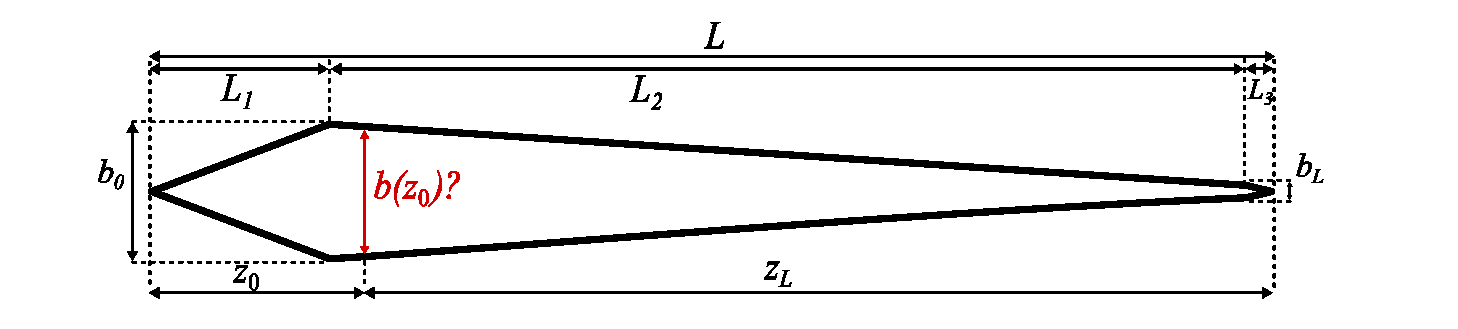
\includegraphics[width=\linewidth]{./images/fffChannelMeasures.pdf}    
  \end{center}
  \caption[Channel dimensions]{Channel dimensions. The width $b(\zL)$ depends on the focus position and is not 
  accessible via geometrical channel data only.}
  \label{fig:fffChannelMeasures} 
\end{figure}AF4 channels have a trapezoidal shape with measures indicated in fig. \ref{fig:fffChannelMeasures}.
For all further considerations, the channel plane is split into three sections (1,2,3) with their correspoding lengths $L_1, L_2, L_3$. To simplify the further calculations, they are subsumed as in the following:
% \begin{itemize}
% \item the widths at the channel intersections
% \item the three lenghts $L_1$, $L_2$ and $L_3$ of the channel sections with their sum
% \end{itemize}
\begin{equation}
  % \dot{L}
  L
  = L_1 + L_2 + L_3 = L_{12} + L_3   
\end{equation}
As the sample is focussed at a certain channel position on the beginning, this has to be considered. The relative focus position \zP is related to the other focus-related magnitudes by
\begin{equation}
  z_0 = \zP L = L - \zL
\end{equation}
The channel height difference \bDelta on the section 2 is
\begin{equation}
  \bDelta = b_0 - \bL \geqq 0
\end{equation}

Volume calculation may be conducted for the trapezoidal by simple decomposition of the channel plane into elementary 
geometrical objects. However, a concise analytical approach is more appropriate as the result can be displayed as a 
function of $\zP$. In addition the corresponding $b(\zP)$ is not known initially. Similar derivations have already been 
conducted with the approximation of dividing the shape into two sections.\cite{Wahlund2013, Magnusson2012, 
Bolinsson2018, Haakansson2012}
The approach may be useful for further hydrodynamic considerations as for example, the elution flow $V_e(x)$ in AF4 is 
a position-dependent size. For the trapezoidal plane shape, the channel is described by the enclosure of three pairs of 
straight line \ref{fig:fffChannelCoordSys}. All expressions here are not optimized for mathematical elegance, but 
rather for being translated into an understandable and well-maintainable calculation routine. This is achieved by 
extensive subsitution of the known variables. Subsuming of these magnitudes helps to simplify the later expressions. 
In addition it allows the transformation and variation if a modification is required, for example if another shape 
model shall be introduced.
Due to the reason of symmetry, only three borders have to be described exactly:

\begin{align}
  \frac{1}{2}b(x) = E(x) \left\{  
  \begin{array}{lcrcl}
    \intGreenBox {\ensuremath{ e_1(x) = m_1 x       = \frac{b_0}{2L_1} \cdot x   }}
    & \forall & 0 \leqq & x &\leqq L_1 \\\addlinespace %\label{eq:chLine1} \\
    \intBlueBox {\ensuremath{ e_2(x) = m_2 x + t_2  = - \frac{\bDelta}{2 L_2} \cdot x  + \frac{1}{2} \left( b_0 +  \frac{L_1}{L_2}\bDelta \right)     }}
    & \forall & L_1 < & x &\leqq L_{12}  \\\addlinespace  % \label{eq:chLine2} \\
    \intPurpleBox {\ensuremath{ e_3(x) = m_3 x + t_3  = - \frac{\bL}{2L_3}  \cdot x + \frac{L \bL}{2 L_3 } }}
    & \forall & L_{12} < & x &\leqq L   \\ %  \label{eq:chLine3}
  \end{array}
  \right.
  \label{eq:chLine}
\end{align}
\begin{figure}  
  \begin{center}
    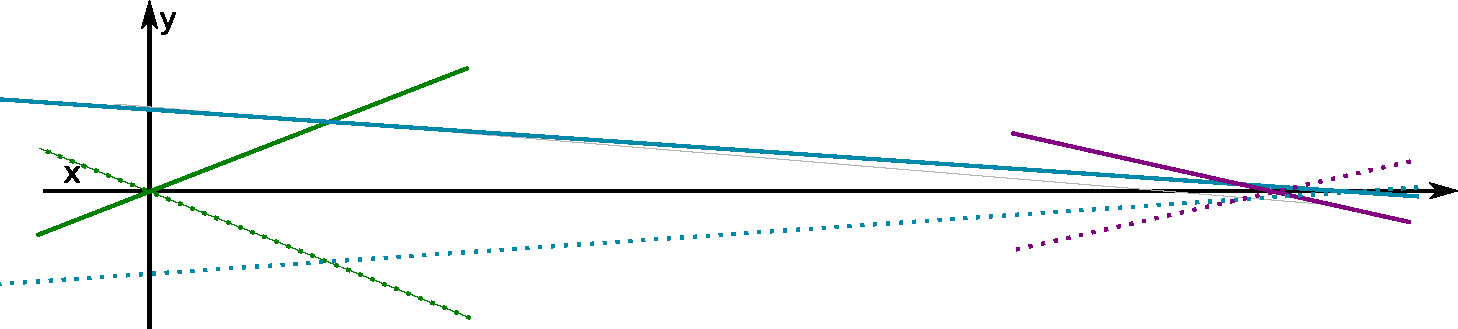
\includegraphics[width=\linewidth]{./images/fffChannelCoordSys.pdf}    
  \end{center}
  \caption[Channel dimensions as a set of straight lines]{Channel dimensions as a set of 3 pairs of straight lines.}
  \label{fig:fffChannelCoordSys} 
\end{figure}
As all dimensions here are known, the slopes and offsets of the lines can be calculated directly and don't have to be resubsituted after the following substitutions.
The calcuation of geometrical volume of the trapezoidal channel has to be adapted according to whether the focus 
position $z_0$ is located left or right to the position of maximal channel extent ( i.e. if $z_0 < L_1$ or $z_0 \geqq 
L_1$). In the algorithm later, rather the plane is used explicitly, which is obtained easily \clearpage
\subsubsection*{\Vgeo: Distal focussing with $\bm{z_0 \geqq L_1}$}
\begin{figure}[h]
  \begin{center}
    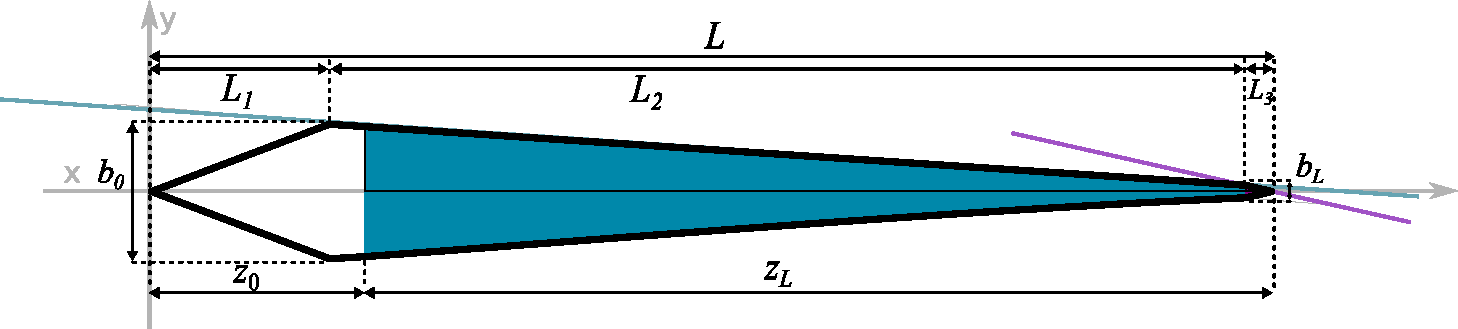
\includegraphics[width=\linewidth]{./images/fffVolume1.pdf}
    \vspace*{-3ex}    
  \end{center}
  \caption[Passed area section - distal focussing]{Area section passed by the sample during the measurement marked with 
  the color of the corresponding line in the case of distal focussing}
  \label{fig:fffVolume1} 
\end{figure}
In this case, the channel volume $\Vgeo$ is the product of the channel width $w$ and the colored area the
$x,y$-plane of Fig. \ref{fig:fffVolume1}.
It is described by:
% \begin{equation}
\begin{align}
  \Vgeo & = &\left(\intBlueBox{\ensuremath{A_2}} + \intPurpleBox{\ensuremath{A_3}}\right) \cdot w \nonumber\\  
        & =&2 \cdot \left( 
             \intBlueBox {\ensuremath{ \int\limits_{z_0}^{L_{12}} e_2(x) \diff x }}
             + \intPurpleBox{\ensuremath{  \int\limits_{L-L_3}^{L} e_3(x) \diff x }}    
             \right) \cdot w  \nonumber \\
        &  =&\left(
              \intBlueBox{\ensuremath{ \left( L_{12}-z_0 \right)  \left( m_2 \left(L_{12}+z_0  \right) + 2 t_2  
              \right)  
              }}
              + \intPurpleBox{\ensuremath{ \frac{1}{2} \cdot L_3 \cdot \bL  } }
              \right) \cdot w
\end{align}

\subsubsection*{\Vgeo: Proximal focussing with $\bm{z_0 < L_1}$}
\begin{figure}[h]
  \begin{center}
    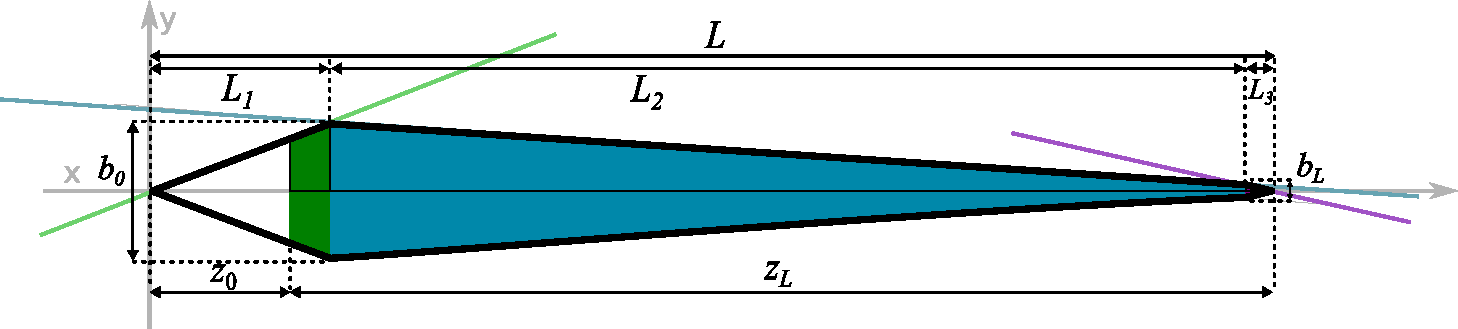
\includegraphics[width=0.95\linewidth]{./images/fffVolume2.pdf}    
  \end{center}
  \vspace*{-3ex}    
  \caption[Passed area section - proximal focussing]{Area section passed by the sample during the measurement marked 
  with the color of the corresponding line in the case of proximal focussing}
  \label{fig:fffVolume2} 
\end{figure}
Outgoing from the previous result, the full area section of section 2 has to be considered, i.e. first $z_0$ is 
replaced by $L_1$, then the area part of section 1 is added:

\begin{align}
  \Vgeo & = &\left( \intGreenBox{\ensuremath{A_1}} +  \intBlueBox{\ensuremath{A_2}} + \intPurpleBox{\ensuremath{A_3}}\right) \cdot w\nonumber \\  
        & =&2 \cdot \left(
             \intGreenBox {\ensuremath{ \int\limits_{z_0}^{L_{1}} e_1(x) \diff x }}
             + \intBlueBox {\ensuremath{ \int\limits_{L_1}^{L_{12}} e_2(x) \diff x }}
             + \intPurpleBox{\ensuremath{  \int\limits_{L-L_3}^{L} e_3(x) \diff x }}    
             \right) \cdot w \nonumber \\
        &  =&\left(
              \intGreenBox {\ensuremath{ m_1 \cdot ( L_1^2 - z_0^2) }}
              + \intBlueBox{\ensuremath{ m_2L_{12}L_2 + m_2L_1L_2 + 2t_2L_2}}{ }
              + \intPurpleBox{\ensuremath{ \frac{1}{2} \cdot L_3 \cdot \bL  } }
              \right) \cdot w   \nonumber\\
        &  =&\left(
              \intGreenBox {\ensuremath{ m_1 \cdot ( L_1^2 - z_0^2) }}
              + \intBlueBox{\ensuremath{   \frac{1}{2} (b_0 + b_L) L_2  }  }{ }
              + \intPurpleBox{\ensuremath{ \frac{1}{2} \cdot L_3 \cdot \bL  } }
              \right) \cdot w         
              \label{eq:proxFocusVolume}
\end{align}

\clearpage
\section*{Determination of ``hydrodynamic" channel height $\bm\whyd$ and Volume $\bm\Vhyd$}
\begin{figure}[h]  
  \begin{center}
    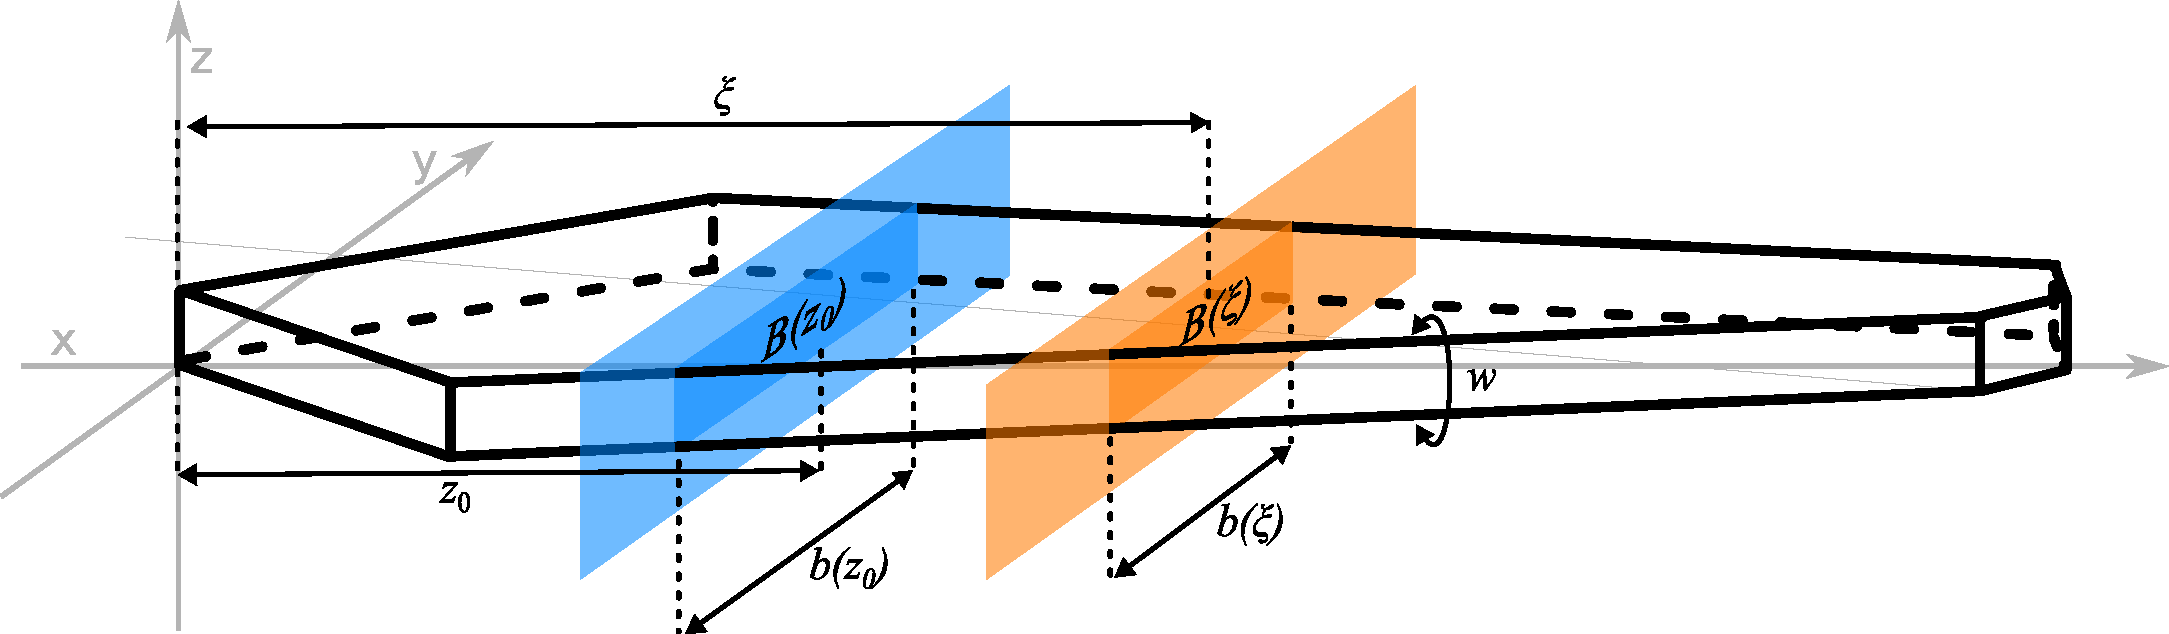
\includegraphics[width=0.95\linewidth]{./images/XiCrossSection.pdf}    
  \end{center}
  \caption[cross sections ]{Cross sections $B(ξ)$ of the channel at different positions $ξ$}
  \label{fig:XiCrossSection} 
\end{figure}
Here, the derivation is analogously conducted as described in literature \scite{Wahlund1987,Litzen1991, Wahlund2013}, 
but using the straight equations \ref{eq:chLine} for description of the channel above. This takes into consideration 
that $b(z)$ is variable over the whole channel length. In addition, also focussing into the first channel section is 
considered, for this reason, the the surface cannot just be corrected by a constant term as reported 
\scite{Litzen1991}. \tvoid is the void time of an unretained species which can be obtained by integration over the 
channel positions $ξ$.
Although this derivation leads to rather laborious expressions, it has the advantage that no additional assumptions are 
necessary. 
\begin{equation}
  \tvoid 
  = \int_0^{\tvoid}  \diff t  
  = \int_{z_0}^{L} \frac{1}{\vm(ξ)} \diff ξ 
  \label{eq:tvoidMigVelo}
\end{equation}
\vm($ξ$) is the migration velocity of the eluent at a channel position $ξ$. It dependends on the flow velocity
$\Vdot(ξ)$ at the position and the $y,z$ cross-sectional area $B(ξ)$  at (Fig \ref{fig:XiCrossSection})
\begin{equation}
  \vm(ξ) = \frac{\Vdot(ξ)}{B(ξ)} = \frac{\Vdot(ξ)}{b(ξ)\cdot w} \label{eq:MigSpeedVXi}
\end{equation}

The term $b(ξ)$ is described with the aid of eq. \ref{eq:chLine} and will require a case-by-case approach.
The change of the flow velocity $\Vdot(ξ)$ is exactly the total loss in the applied crossflow. It has its maximum at the inlet position with
\begin{equation}
  \Vdot(0) = \Vin = \Ve + \Vc
  \label{eq:DefVin}
\end{equation}
and its minimum with
\begin{equation}
  \Vdot(L) = \Ve       
\end{equation}
As this is distributed uniformly over the membrane surface, the decay is proportional to the area the eluent has already passed. This leads to the expression
\begin{equation}
  \Vdot(ξ) = \Vin - V_c \cdot \frac{A(ξ)}{\AL}    
  = \Vin - V_c \cdot \ddfrac{ \int_0^{ξ}b(x) \diff x }{ \int_0^{L}b(x) \diff x   }   
  = \Vin - V_c \cdot \ddfrac{2 \cdot \int_0^{ξ}E(x) \diff x }{ \AL  }
  \label{eq:VDepXi}
\end{equation}
The total area \AL can be easily derived by letting of eq. \ref{eq:proxFocusVolume} with letting $z_0 = 0$:
\begin{equation}
  \begin{array}{ll}
    \AL =\intGreenBox{\ensuremath{A_1}} +  \intBlueBox{\ensuremath{A_2}} + \intPurpleBox{\ensuremath{A_3}} % \left(
    &= \intGreenBox {\ensuremath{ \frac{1}{2} b_0  L_1  }}
      + \intBlueBox{\ensuremath{ \frac{1}{2} (b_0 + b_L) L_2  }}
      + \intPurpleBox{\ensuremath{ \frac{1}{2} L_3\bL  } }
      % \right)
      % \cd      
  \end{array}
  \label{eq:areaSections}
\end{equation}
To evaluate $A(ξ)$ correctly, the integrals have to be split according to the conditions in eq. \ref{eq:chLine}. This 
is required which corresponds to the cases needed for $b(ξ)$.
Merging eq. \ref{eq:tvoidMigVelo}
and \ref{eq:VDepXi} gives the expression
\begin{equation}
  \vm(ξ) = \dfrac{\Vin - V_c \cdot \frac{2 \cdot \int_0^{ξ}E(x) \diff x }{  \AL }}{ 2\cdot E(ξ) \cdot w  } 
  =\frac{1}{2\cdot w } \cdot \frac{\Vin - V_c \cdot \frac{2 \cdot \int_0^{ξ}E(x) \diff x }{ \AL }}{ E(ξ)}
\end{equation}
Inserting into eq. \ref{eq:tvoidMigVelo} gives:
\begin{equation}
  \tvoid = 2 \cdot w \cdot 
  \int_{z_0}^{L} 
  %\left(
   \ddfrac{ E(ξ) }{  \Vin - V_c \cdot \frac{2 \cdot \int_0^{ξ}E(x) \diff x }{ \AL  }  }
    %\right)
     \diff ξ
  \label{eq:awfulIntegrals}
\end{equation}
This expression quantifies a linear conversion factor $\CF$ for the relationship of  \tvoid\ and $w$. This promises a simple relationship between those two basic magnitudes with
\begin{equation}
  \tvoid = 2 \cdot \CF \cdot w
\end{equation}
and
\begin{equation}
  \CF = \int_{z_0}^{L}
  % \left(  
   \ddfrac{ E(ξ) }{ \Vin - V_c \cdot \dfrac{2 \cdot \int_0^{ξ}E(x) \diff x }{ \AL  }  
   } 
 %\right)
  \diff ξ
\end{equation}
Similar to the calculation of \Vgeo above, a case-by case analysis is required depending on $z_0$. Due to the 
section-wise definition of the integrand, the integrals then have to be split accordingly to the partial domain of 
$E(ξ)$.
\clearpage
\subsubsection*{\Vhyd: Distal focussing with $\bm{z_0 \geqq L_1}$}
  Here, the outer integral of eq. \ref{eq:awfulIntegrals} is split into the sections with  $L_1 < ξ \leqq L_{12}$ 
  and  $L_{12} < ξ$:
  % \begin{equation}
\begin{equation}
  \CF =
    \int_{z_0}^{L_{12}}  
    %\left(
      \ddfrac{ E(ξ) }{ \Vin - \frac{2V_c}{ \AL }  \int_0^{ξ}E(x) \diff x  }
     %  \right)
        \diff ξ
    +  \int_{L_{12}}^{L}
    % \left(
      \ddfrac{ E(ξ) }{ \Vin - \frac{2V_c}{ \AL  } \int_0^{ξ}E(x) \diff x  }
      % \right)
       \diff ξ 
  % \label{}
\end{equation}
As  $ξ$ is now located only on one of the section within each summand, the inner integrals can be split for the 
different domains of $E(x)$. Integrals independent from $ξ$ are directly substituted with their corresponding area 
section from eq. \ref{eq:areaSections}, only the last integral is solved.
% \end{equation}
% \begin{equation}
\begin{equation}
  \begin{array}{lllll}
    \CF &=
    &%\left( \vphantom{\ddfrac{dummy}{\int_a^b}} \right. % phantom bracket^^
    &&\displaystyle\int_{z_0}^{L_{12}}
    % \left(
       \ddfrac{  e_2(ξ)    }{   \Vin - \frac{2V_c}{ \AL  }
       \left(
       \int_0^{L_1}e_1(x) \diff x
       + \int_{L_1}^{ξ}e_2(x) \diff x
       \right)      
       }
       \diff ξ
    \\    
        &&&+& \displaystyle\int_{L_{12}}^{L}              
              \ddfrac{ e_3(ξ)  }{   \Vin - \frac{2V_c}{ \AL  }
              \left(
              \int_0^{L_1}e_1(x) \diff x
              + \int_{L_1}^{L_{12}}e_2(x) \diff x
              + \int_{L_{12}}^{ξ}e_3(x) \diff x
              \right)    
              }
              \diff ξ
              % \left.  \vphantom{\ddfrac{dummy}{\int_a^b}}   \right) %% phantom bracket^^
    \\\addlinespace[4ex]        
        &=
    &%\left( \vphantom{\ddfrac{dummy}{\int_a^b}} \right.
    &&\displaystyle\int_{z_0}^{L_{12}}
       
       \ddfrac{   m_2 \cdot ξ + t_2   }{   \Vin - \frac{2V_c}{ \AL  }
       \left(
       \frac{1}{2} A_1
       + \frac{1}{2} m_2 ( ξ^2 - L_1^2 )   + t_2( ξ - L_1 )               
       \right)
       }
       \diff ξ\\
        &&&+& \displaystyle\int_{L_{12}}^{L}
              \ddfrac{    m_3 \cdot ξ + t_3  }{   \Vin - \frac{2V_c}{ \AL  }
              \left(
              \frac{1}{2} A_1
              + \frac{1}{2} A_2 
              + \frac{1}{2} m_3 ( ξ^2 - L_{12}^2 )   + t_3( ξ - L_{12} )          
              \right)             
              }
              \diff ξ
              % \left. \vphantom{\ddfrac{dummy}{\int_a^b}}  \right) %% phantom bracket^^
    \\
  \end{array}
  % \label{}
\end{equation}
In order to transform the integrand terms into ordinary rational functions and simplify the analytical solutions 
This can be rearranged by using substitutions for the occurring prefactors $α_i,β_i,γ_i,δ_i$, the quadratic polynomials 
$P(ξ)$ and its discriminants
$Δ_i$:
\begin{equation}
  \begin{array}{lllll}
    α_2 = \frac{t_2}{m_2}
    & β_2 = -\frac{\Vc m_2}{ \AL }
    & γ_2 = -\frac{2 \Vc t_2}{\AL}\\\addlinespace
    \multicolumn{3}{l}{ δ_2 = \Vin - \frac{\Vc}{\AL} \left( A_1 - m_2L_1^2 - 2t_2L_1  \right) }
    & Δ_2 =4β_2 δ_2 - γ_2^2
    \\\addlinespace[2ex]
    α_3 = \frac{t_3}{m_3}
    &β_3 = -\frac{\Vc m_3}{ \AL }
    &γ_3 = -\frac{2 \Vc t_3}{\AL}\\\addlinespace
    \multicolumn{3}{l}{ δ_3 =\Vin - \frac{\Vc}{\AL} \left( A_1 + A_2 - m_3L_{12}^2 - 2t_3L_{12}  \right) }
    & Δ_3 =  4β_3 δ_3 - γ_3^2
  \end{array}%{lllllllll}
\end{equation}
\begin{equation}
  \begin{array}{ll}
    P_2(ξ) = β_2 ξ^2 + γ_2 ξ + \delta_2\\\addlinespace[2ex]
    P_3(ξ) = β_3 ξ^2 + γ_3 ξ + \delta_3
  \end{array}
\end{equation}
  For solving the integral it is important to know the sign of $\Delta_2$ and $\Delta_3$. Inserting \ref{eq:DefVin}, it 
  can be shown (see below) that it is not possible to determine the scope of $\Delta_2$ exactly for the general case 
  and the case-by-case analysis has to be conducted ``at runtime''. To simplify the display of this expression, it 
  is split and each summand treated separately:
      \begin{equation}
  \CF = \CFtwo +\CFthree  
\end{equation}
\begin{equation}
  \begin{array}{lllll}
    \CFtwo &= 
    &   m_2 \cdot \displaystyle\int_{z_0}^{L_{12}}  
      \ddfrac{    ξ + α_2   }{
      β_2 ξ^2 + γ_2 ξ + \delta_2
      }
      \diff ξ \\\addlinespace
      %%%%%%%%%%%%%%%%%%%%% 
           &= 
    &   m_2 \cdot
      \left(
      \displaystyle\int_{z_0}^{L_{12}}       
      \ddfrac{ ξ }{
      P_2(ξ) % β_2 ξ^2 + γ_2 ξ + \delta_2
      }
      \diff ξ
      +
      \displaystyle\int_{z_0}^{L_{12}}       
      \ddfrac{ α_2 }{
      P_2(ξ) % β_2 ξ^2 + γ_2 ξ + \delta_2
      }
      \diff ξ
      \right)     \\\addlinespace
      %%%%%%%%%%%%%%%%%%%%%%% 
           &=
    &m_2 \cdot
      \left(
      \left[    \frac{\ln{P_2(ξ)}}{2β_2} \right]_{z_0}^{L_{12}}

      + 
      \left(
      α_2 - \frac{γ_2}{2β_2}
      \right)
      \displaystyle\int_{z_0}^{L_{12}}       
      \ddfrac{\diff ξ }{
      P_2(ξ) % β_2 ξ^2 + γ_2 ξ + \delta_2
      }             
      \right) & \scite{Bronstein2008}
    \\\addlinespace
           &=
    &\begin{cases}
      %%%%%%%%%%%%%%%%%%%%%%% 
      \mathrlap{
        m_2 \cdot
        \left(
          \left[ \frac{\ln{P_2(ξ)}}{2β_2} \right]_{z_0}^{L_{12}}
          + 
          \left(
            α_2 - \frac{γ_2}{2β_2}
          \right)
          \left[
            \ddfrac{2}{\sqrt{Δ_2}} \cdot \text{arctan}{\left( \ddfrac{ \displaystyle 2β_2\xi+γ_2 }{\displaystyle 
            \sqrt{Δ_2} } \right) }
          \right]_{z_0}^{L_{12}}
        \right)
      }
      \phantom{      m_2 \cdot \left(\frac{1}{2β_2}\ln{\frac{P_2(L_{12})}{ P_2(z_0)}}-\left(\frac{2}{\sqrt{-Δ_2}}\right)\left(α_2 - \frac{γ_2}{2β_2}\right)\left(\text{artanh}\ddfrac{2β_2 (L_{12} - z_0)}{\left(\sqrt{-Δ_2}- \scriptstyle
                \frac{ \left(2β_2L_{12}+γ_2 \right)  \left(2β_2z_0+γ_2 \right) }{\sqrt{-Δ_2}}\right)}\right)\right)                  }    
      & \forall Δ_2 > 0
      \\\addlinespace
      m_2 \cdot
      \left(
        \left[ \frac{\ln{P_2(ξ)}}{2β_2} \right]_{z_0}^{L_{12}}
        + 
        \left(
          α_2 - \frac{γ_2}{2β_2}
        \right)
        \left[
          -\ddfrac{2}{\sqrt{-Δ_2}} \cdot \text{artanh}{\left( \ddfrac{ 2β_2\xi+γ_2 }{ \sqrt{-Δ_2} } \right) }
        \right]_{z_0}^{L_{12}} 
      \right) & \forall Δ_2 < 0 \\\addlinespace
    \end{cases} & \scite{Bronstein2008a}
    %%%%%%%%%% 
    \\\addlinespace
           &=
    &\begin{cases}
      \mathrlap{
        m_2 \cdot \Bigg(
        \frac{1}{2β_2}
        \Big(\scriptstyle
        \ln{P_2(L_{12})} - \ln{P_2({z_0})}
        \Big)
        +
        \left(
          \frac{2}{\sqrt{Δ_2}}
        \right)
        \left(
          α_2 - \frac{γ_2}{2β_2}
        \right)
        \left(
          \text{arctan} \ddfrac{ 2β_2L_{12}+γ_2 }{ \sqrt{Δ_2} }
          - \text{arctan} \ddfrac{ 2β_2z_0+γ_2 }{ \sqrt{Δ_2} }
        \right)        
        \Bigg)
      }
      \phantom{      m_2 \cdot \left(\frac{1}{2β_2}\ln{\frac{P_2(L_{12})}{ P_2(z_0)}}-\left(\frac{2}{\sqrt{-Δ_2}}\right)\left(α_2 - \frac{γ_2}{2β_2}\right)\left(\text{artanh}\ddfrac{2β_2 (L_{12} - z_0)}{\left(\sqrt{-Δ_2}- \scriptstyle
                \frac{ \left(2β_2L_{12}+γ_2 \right)  \left(2β_2z_0+γ_2 \right) }{\sqrt{-Δ_2}}\right)}\right)\right)                  }
      & \forall Δ_2 > 0\\\addlinespace
      m_2 \cdot \Bigg(
      % \left(
      \frac{1}{2β_2}
      \Big(\scriptstyle
      \ln{P_2(L_{12})} - \ln{P_2({z_0})}
      \Big)
      -
      \left(
        \frac{2}{\sqrt{-Δ_2}}
      \right)
      \left(
        α_2 - \frac{γ_2}{2β_2}
      \right)
      \left(
        \text{artanh} \ddfrac{ 2β_2L_{12}+γ_2 }{ \sqrt{-Δ_2} }
        - \text{artanh} \ddfrac{ 2β_2z_0+γ_2 }{ \sqrt{-Δ_2} }
      \right)
      % \right)
      \Bigg) & \forall Δ_2 < 0 
    \end{cases} 
    %%%%%%%%%% 
    \\\addlinespace
           &=
    &\begin{cases}
      \mathrlap{
        m_2 \cdot \left(
          \frac{1}{2β_2}       
          \ln{\frac{P_2(L_{12})}{ P_2(z_0)}}
          +
          \left(
            \frac{2}{\sqrt{Δ_2}}
          \right)
          \left(
            α_2 - \frac{γ_2}{2β_2}
                \right)
            \left(
              \text{arctan} \ddfrac{ 2β_2L_{12}+γ_2 }{ \sqrt{Δ_2} }
              - \text{arctan} \ddfrac{ 2β_2z_0+γ_2 }{ \sqrt{Δ_2} }            
          \right)
        \right)
      }\phantom{      m_2 \cdot \left(\frac{1}{2β_2}\ln{\frac{P_2(L_{12})}{ P_2(z_0)}}-\left(\frac{2}{\sqrt{-Δ_2}}\right)\left(α_2 - \frac{γ_2}{2β_2}\right)\left(\text{artanh}\ddfrac{2β_2 (L_{12} - z_0)}{\left(\sqrt{-Δ_2}- \scriptstyle
                \frac{ \left(2β_2L_{12}+γ_2 \right)  \left(2β_2z_0+γ_2 \right) }{\sqrt{-Δ_2}}\right)}\right)\right)                  }    
      & \forall Δ_2 > 0
      \\\addlinespace
      m_2 \cdot \left(
        \frac{1}{2β_2}       
        \ln{\frac{P_2(L_{12})}{ P_2(z_0)}}
        -
        \left(
          \frac{2}{\sqrt{-Δ_2}}
        \right)
        \left(
          α_2 - \frac{γ_2}{2β_2}
        \right)
        \left(          
          \text{artanh}
          \frac{2β_2L_{12}+ γ_2 - 2β_2z_0-γ_2
          }{
            \sqrt{-Δ_2} \cdot \left(
              1 - \scriptstyle
              \frac{2β_2L_{12}+γ_2 }{ \sqrt{-Δ_2} } \cdot
              \frac{2β_2z_0+γ_2 }{ \sqrt{-Δ_2} }
            \right)

          }
        \right)        
      \right)
      & \forall Δ_2 < 0 
    \end{cases}
    \\\addlinespace
    %%%%%%%%%%%%%%%%%%% 
           &= &\begin{cases}
             m_2 \cdot \left(
               \frac{1}{2β_2}       
               \ln{\frac{P_2(L_{12})}{ P_2(z_0)}}
               +
               \left(
                 \frac{2}{\sqrt{Δ_2}}
               \right)
               \left(
                 α_2 - \frac{γ_2}{2β_2}
                  \right) 
                 \left(
                   \text{arctan} \ddfrac{ 2β_2L_{12}+γ_2 }{ \sqrt{Δ_2} }
                   - \text{arctan} \ddfrac{ 2β_2z_0+γ_2 }{ \sqrt{Δ_2} }                   
               \right)
             \right)
             & \forall Δ_2 > 0\\\addlinespace
             m_2 \cdot \left(
               \frac{1}{2β_2}       
               \ln{\frac{P_2(L_{12})}{ P_2(z_0)}}
               -
               \left(
                 \frac{2}{\sqrt{-Δ_2}}
               \right)
               \left(
                 α_2 - \frac{γ_2}{2β_2}
               \right)
               \left(
                 \text{artanh}
                 \ddfrac{2β_2 (L_{12} - z_0)
                 }{
                   \left(
                     \sqrt{-Δ_2}- \scriptstyle
                     % \frac{2β_2L_{12}+γ_2 }{ \sqrt{-Δ_2} } \cdot
                     \frac{ \left(2β_2L_{12}+γ_2 \right)  \left(2β_2z_0+γ_2 \right) }{\sqrt{-Δ_2}}
                     % \frac{2β_2z_0+γ_2 }{ \sqrt{-Δ_2} }
                   \right)
                 }
               \right)        
             \right)    & \forall Δ_2 < 0 
           \end{cases}                
  \end{array}    \label{eq:CFtwo}  
\end{equation}

\begin{equation}
  \begin{array}{lclll}
    \CFthree &=
    & m_3 \cdot \displaystyle\int_{L_{12}}^{L}
      \ddfrac{   ξ + α_3
      }{
      β_3 ξ^2 + γ_3 ξ + \delta_3
      }
      \diff ξ \\\addlinespace
             & =&  m_3 \cdot
                  \left(
                  \displaystyle\int_{L_{12}}^{L}       
                  \ddfrac{ ξ }{
                  P_3(ξ) % β_2 ξ^2 + γ_2 ξ + \delta_2
                  }
                  \diff ξ
                  +
                  \displaystyle\int_{L_{12}}^{L}       
                  \ddfrac{ α_3 }{
                  P_3(ξ) % β_2 ξ^2 + γ_2 ξ + \delta_2
                  }
                  \diff ξ
                  \right)
                  % \right)
    \\\addlinespace[2ex]
             &&    \cdots\ \text{analogously to eq. \ref{eq:CFtwo} }\cdots    \\\addlinespace[2ex]
             &=
    & \begin{cases}
      m_3 \cdot \left(
        \frac{1}{2β_3}       
        \ln{\frac{P_3(L)}{ P_3(L_{12})}}
        +
        \left(
          \frac{2}{\sqrt{Δ_3}}
        \right)
        \left(
          α_3 - \frac{γ_3}{2β_3}
           \right)  
          \left(
            \text{arctan} \ddfrac{ 2β_3L+γ_3 }{ \sqrt{Δ_3} }
            - \text{arctan} \ddfrac{ 2β_3L_{12}+γ_3 }{ \sqrt{Δ_3} }           
        \right)
      \right)
      & \forall Δ_3 > 0\\\addlinespace
      m_3 \cdot \left(
        \frac{1}{2β_3}       
        \ln{\frac{P_3(L)}{ P_3(L_{12})}}
        -
        \left(
          \frac{2}{\sqrt{-Δ_3}}
        \right)
        \left(
          α_3 - \frac{γ_3}{2β_3}
        \right)
        \left(
          \text{artanh}
          \ddfrac{2β_3 (L - L_{12})
          }{
            \left(
              \sqrt{-Δ_3}- \scriptstyle
              % \frac{2β_2L_{12}+γ_2 }{ \sqrt{-Δ_2} } \cdot
              \frac{ \left(2β_3L+γ_3 \right)  \left(2β_3L_{12}+γ_3 \right) }{\sqrt{-Δ_3}}
              % \frac{2β_2z_0+γ_2 }{ \sqrt{-Δ_2} }
            \right)

          }
        \right)        
      \right)    & \forall Δ_3 < 0
      %%%%%%%%%%%%%%%%%%%%%       
    \end{cases}
  \\\addlinespace[2ex]
             &=
    & \begin{cases}
      m_3 \cdot \left(
        \frac{1}{2β_3}
        \ln{\frac{P_3(L)}{ P_3(L_{12})}}
        +
        \left(
          \frac{2}{\sqrt{Δ_3}}
        \right)
        \left(
          α_3 - \frac{γ_3}{2β_3}
          \right) 
          \left(
            \text{arctan} \ddfrac{ 2β_3L+γ_3 }{ \sqrt{Δ_3} }
            - \text{arctan} \ddfrac{ 2β_3L_{12}+γ_3 }{ \sqrt{Δ_3} }             
        \right)
      \right)
      & \forall Δ_3 > 0\\\addlinespace
      m_3 \cdot \left(
        \frac{1}{2β_3}       
        \ln{\frac{P_3(L)}{ P_3(L_{12})}}
        -
        \left(
          \frac{2}{\sqrt{-Δ_3}}
        \right)
        \left(
          α_3 - \frac{γ_3}{2β_3}
        \right)
        \left(
          \text{artanh}
          \ddfrac{2β_3\left( L- L_{12} \right)
          }{
            \left(
              \sqrt{-Δ_3}- \scriptstyle
              % \frac{2β_2L_{12}+γ_2 }{ \sqrt{-Δ_2} } \cdot
              \frac{ \left(2β_3L+γ_3 \right)  \left(2β_3L_{12}+γ_3 \right) }{\sqrt{-Δ_3}}
              % \frac{2β_2z_0+γ_2 }{ \sqrt{-Δ_2} }
            \right)            
          }
        \right)        
      \right)    & \forall Δ_3 < 0
    \end{cases}
  \end{array}
\end{equation}
\clearpage
% The last expression can be easily evaluated and needs only to call 6 numerical subroutines (which would be relevant if it was embedded into an algorithm with numerous calls of this calculation).
\subsubsection*{\Vhyd: Proximal focusing with $\bm{z_0 < L_1}$}
If the sample was focused to a point with $z_0 < L_1$, the in addition to the solution above, also the eluent migration 
through the first sections has to be considered. The evaluation of the expression can be conducted analogously for the 
second and third summand as shown above with adaption of the lower limit of integration for the second:
\begin{equation}
  \begin{array}{lcll}
    \CF
    &=      
    &     % \left(% \vphantom{\ddfrac{dummy}{\int_a^b}} \right.
    &\displaystyle\int_{z_0}^{L_{1}}  \ddfrac{  e_1(ξ)  }{   \Vin - \frac{2V_c}{ \AL  }
      \left(
      \int_0^{ξ}e_1(x) \diff x
      \right)
      }  \diff ξ\\
    &&+&  \displaystyle\int_{L_1}^{L_{12}}    \ddfrac{  e_2(ξ)  }{   \Vin - \frac{2V_c}{ \AL  }
         \left(
         \int_0^{L_1}e_1(x) \diff x
         + \int_{L_1}^{ξ}e_2(x) \diff x
         \right) }
         \diff ξ\\
    &&+& \displaystyle\int_{L_{12}}^{L} %\left(
         \ddfrac{   e_3(ξ)  }{   \Vin - \frac{2V_c}{ \AL  }
         \left(
         \int_0^{L_1}e_1(x) \diff x
         + \int_{L_1}^{L_{12}}e_2(x) \diff x
         + \int_{L_{12}}^{ξ}e_3(x) \diff x
         \right)    }
         \diff ξ
         % \left. \vphantom{\ddfrac{dummy}{\int_a^b}}          \right)%% phantom bracket^^
    \\   
    &=      
    &%2 \cdot w \cdot
    % \left(
    %   \vphantom{\ddfrac{dummy}{\int_a^b}} \right.
    &\displaystyle\int_{z_0}^{L_{1}}  \ddfrac{  m_1 \cdot ξ  }{   \Vin - \frac{2V_c}{ \AL  }
      \left(
      \frac{1}{2} m_1 ξ^2  
      \right)
      } \diff ξ\\
    &&+&  \displaystyle\int_{L_1}^{L_{12}}    \ddfrac{ m_2 \cdot ξ + t_2 }{   \Vin - \frac{2V_c}{ \AL  }
         \left(
         \frac{1}{2} A_1
         + \frac{1}{2} m_2 ( ξ^2 - L_1^2 )   + t_2( ξ - L_1 ) 
         \right)
         } \diff ξ\\
    &&+& \displaystyle\int_{L_{12}}^{L}  \ddfrac{  m_3 \cdot ξ + t_3   }{   \Vin - \frac{2V_c}{ \AL  }
         \left(
         \frac{1}{2} A_1 
         + \frac{1}{2} A_2    
         + \frac{1}{2} m_3 ( ξ^2 - L_{12}^2 )   + t_3( ξ - L_{12} )   
         \right)    
         } \diff ξ
         % \left. \vphantom{\ddfrac{dummy}{\int_a^b}}  \right)%% phantom bracket^^
    \\
  \end{array}
\end{equation}

Substitution is done similarly as above:
\begin{equation}  
  \begin{array}{lllll}
    & β_1 = -\frac{\Vc m_1}{ \AL }
    & δ_1 = \Vin   %\frac{2 \Vc t_1}{\AL}
    \\\addlinespace
    α_2 = \frac{t_2}{m_2}
    & β_2 = -\frac{\Vc m_2}{ \AL }
    & γ_2 = -\frac{2 \Vc t_2}{\AL}\\\addlinespace
    \multicolumn{3}{l}{ δ_2 = \Vin - \frac{\Vc}{\AL} \left( A_1 - m_2L_1^2 - 2t_2L_1  \right) }
    & Δ_2 =4β_2 δ_2 - γ_2^2
    \\\addlinespace[2ex]
    α_3 = \frac{t_3}{m_3}
    &β_3 = -\frac{\Vc m_3}{ \AL }
    &γ_3 = -\frac{2 \Vc t_3}{\AL}\\\addlinespace
    \multicolumn{3}{l}{ δ_3 =\Vin - \frac{\Vc}{\AL} \left( A_1 + A_2 - m_3L_{12}^2 - 2t_3L_{12}  \right) }
    & Δ_3 =  4β_3 δ_3 - γ_3^2
  \end{array}%{lllllllll}
\end{equation}
\begin{equation}
  \begin{array}{ll}
    P_2(ξ) = β_2 ξ^2 + γ_2 ξ + \delta_2\\\addlinespace[2ex]
    P_3(ξ) = β_3 ξ^2 + γ_3 ξ + \delta_3
  \end{array}
\end{equation}
\clearpage
Then, in analogy, to the case $z_0 \geqq L_1$, $\CF$ can be expressed as 
\begin{equation}
  \begin{array}{lcll}
    \CF  &= &\CFone + \CFtwo + \CFthree\\
         & =    
            &&       
       m_1 \cdot \displaystyle\int_{z_0}^{L_{1}}
       \left(
       \ddfrac{
       ξ 
       }{
       β_1 \cdot ξ^2 + δ_1
       } \right) \diff ξ
    \\\addlinespace
        &&+& m_2 \cdot \displaystyle\int_{L_1}^{L_{12}} \left(
             \ddfrac{
             ξ + α_2         
             }{
             β_2 ξ^2 + γ_2 ξ + δ_2          
             } \right) \diff ξ
    \\\addlinespace
        &&+& m_3 \cdot \displaystyle\int_{L_{12}}^{L} \left(
             \ddfrac{
             ξ + α_3        
             }{
             β_3 ξ^2 + γ_3 ξ + δ_3 
             } \right) \diff ξ
  \end{array}
  % \label{}
\end{equation}
with
%%%% CF1
\begin{equation}
  \begin{array}{lcll}
    \CFone &=
    & m_1 \cdot \displaystyle\int_{z_0}^{L_{1}}
      \left(
      \ddfrac{
      ξ 
      }{
      β_1 \cdot ξ^2 + δ_1
      } \right) \diff ξ
    \\ \addlinespace[1ex]
    &= & \frac{ m_1}{ β_1} \cdot \displaystyle\int_{z_0}^{L_{1}}
    \left(
    \frac{
    ξ 
    }{
    \scriptstyle \frac{δ_1}{β_1} + \displaystyle ξ^2 W 
  } \right) \diff ξ
  \\ \addlinespace[1ex]
     &= &\ddfrac{ m_1}{ β_1} \cdot \frac{1}{2}
     \left[
       \ln(\left| \ddfrac{δ_1}{β_1} + \displaystyle ξ^2 \right|)
     \right]_{z_0}^{L_{1}} %& \scite{Bronstein2008b}
   \\ \addlinespace[1ex]
  &= &\ddfrac{ m_1}{2 β_1} \cdot 
    \left(
      \ln \left| \ddfrac{δ_1}{β_1} + \displaystyle L_1^2 \right| 
      -
      \ln \left| \ddfrac{δ_1}{β_1} + \displaystyle z_0^2 \right| 
    \right)
  \end{array}
  % \label{}
\end{equation}
%%%% CF2
\begin{equation}
  \begin{array}{lclll}
    \CFtwo &= &\begin{cases}
      m_2 \cdot \left(
        \frac{1}{2β_2}       
        \ln{\frac{P_2(L_{12})}{ P_2(L_1)}}
        +
        \left(
          \frac{2}{\sqrt{Δ_2}}
        \right)
        \left(
          α_2 - \frac{γ_2}{2β_2}
       \right)    
          \left(
            \text{arctan} \ddfrac{ 2β_2L_{12}+γ_2 }{ \sqrt{Δ_2} }
            - \text{arctan} \ddfrac{ 2β_2L_1+γ_2 }{ \sqrt{Δ_2} }
        \right)
      \right)
             & \forall Δ_2 > 0\\\addlinespace
             m_2 \cdot \left(
               \frac{1}{2β_2}       
               \ln{\frac{P_2(L_{12})}{ P_2(L_1)}}
               -\left(
                 \frac{2}{\sqrt{-Δ_2}}
               \right)
               \left(
                 α_2 - \frac{γ_2}{2β_2}
               \right)
               \left(
                 \text{artanh}
                 \ddfrac{2β_2 (L_{12} - L_1)
                 }{
                   \left(
                     \sqrt{-Δ_2}- \scriptstyle
                     % \frac{2β_2L_{12}+γ_2 }{ \sqrt{-Δ_2} } \cdot
                     \frac{ \left(2β_2L_{12}+γ_2 \right)  \left(2β_2z_0+γ_2 \right) }{\sqrt{-Δ_2}}
                     % \frac{2β_2z_0+γ_2 }{ \sqrt{-Δ_2} }
                   \right)                   
                 }
               \right)        
             \right)    & \forall Δ_2 < 0 
           \end{cases}                
  \end{array}
\end{equation}


%%%% CF3

\begin{equation}
  \begin{array}{lclll}
    \CFthree &=    & \begin{cases}
      m_3 \cdot \left(
        \frac{1}{2β_3}       
        \ln{\frac{P_3(L)}{ P_3(L_{12})}}
        +
        \left(
          \frac{2}{\sqrt{Δ_3}}
        \right)
        \left(
          α_3 - \frac{γ_3}{2β_3}
           \right)
          \left(
            \text{arctan} \ddfrac{ 2β_3L+γ_3 }{ \sqrt{Δ_3} }
            - \text{arctan} \ddfrac{ 2β_3L_{12}+γ_3 }{ \sqrt{Δ_3} }             
        \right)
      \right)
      & \forall Δ_3 > 0\\\addlinespace
      m_3 \cdot \left(
        \frac{1}{2β_3}       
        \ln{\frac{P_3(L)}{ P_3(L_{12})}}
        -\left(
          \frac{2}{\sqrt{-Δ_3}}
        \right)
        \left(
          α_3 - \frac{γ_3}{2β_3}
        \right)
        \left(
          \text{artanh}
          \ddfrac{2β_3\left( L- L_{12} \right)
          }{
            \left(
              \sqrt{-Δ_3}- \scriptstyle
              % \frac{2β_2L_{12}+γ_2 }{ \sqrt{-Δ_2} } \cdot
              \frac{ \left(2β_3L+γ_3 \right)  \left(2β_3L_{12}+γ_3 \right) }{\sqrt{-Δ_3}}
              % \frac{2β_2z_0+γ_2 }{ \sqrt{-Δ_2} }
            \right)            
          }
        \right)        
      \right)    & \forall Δ_3 < 0
    \end{cases}
  \end{array}
  % \label{}
\end{equation}
                                                           
 \subsubsection*{Evaluation of $\bm \Delta_2$}
To avoid an additional case-by-case analysis for the integration, the discriminants the polynomials $P_2(ξ)$ and $P_3(ξ)$ each were resubsituted to derive that only one of the cases
\[
  \int \frac{\diff ξ}{β_i ξ^2 + γ_i ξ + δ_i}
  \left\{  
    \begin{array}{llll}
      = \ddfrac{2}{\sqrt{Δ_i}} \cdot \arctan{\left( \ddfrac{ 2β_iξ_i+γ_i }{ \sqrt{Δ_i} } \right) }
      & \forall &  Δ_i > 0  \\\addlinespace %\label{eq:chLine1} \\
      = - \ddfrac{2}{\sqrt{-Δ_i}} \cdot \text{artanh}{\left( \ddfrac{ 2β_iξ_i+γ_i }{ \sqrt{-Δ_i} } \right)}
      & \forall & Δ_i < 0  \\ %  \label{eq:chLine3}
    \end{array}
  \right. \qquad\ \scite{Bronstein2008a}
  % \label{eq:chLine}
  % end{align}  
\]
has to be applied for the evaluation of $\CF$:\clearpage
%%%%%%%%%%%%%%%%%%%%%%%%% 
%\vspace*{2ex}\\
%$\bm{z_0 \geqq L_1}$\\
\begin{equation}
  \begin{array}{lll}
    Δ_2
    &=  4β_2δ_2 - γ_2^2      
    \\\addlinespace
    &= 
      4 \cdot \left(- \frac{\Vc m_2}{\AL} \right) \cdot
      \left(
      \Vin - \frac{\Vc}{\AL} \left(  A_1 - m_2L_1^2 - 2t_2L_1 \right)
      \right)
      -\left( - \frac{2 \Vc t_2}{\AL} \right)^2
    \\\addlinespace
    &=     
      - 4 \cdot \frac{\Vc m_2 \Vin}{\AL}
      + 4\cdot \frac{\Vc^2m_2A_1}{\AL^2}
      - 4\cdot \frac{\Vc^2m_2^2L_1^2}{\AL^2}
      - 4\cdot \frac{2 \Vc^2m_2 t_2 L_1}{\AL^2}
      - 4 \cdot \frac{\Vc^2t_2^2}{\AL^2}
    \\\addlinespace   
    &=
      \left( 4 \cdot \frac{\Vc^2}{\AL^2} \right)
      \cdot \left(- m_2A_1 + m_2^2L_1^2 - 2 m_2t_2L_1 -t_2^2  \right)      
      - 4 \cdot \frac{\Vc m_2 \Vin}{\AL}
    \\\addlinespace
    &=
      \left( \frac{\Vc^2}{\AL^2} \right)
      \cdot \left(
      -   \frac{L_1}{L_2} b_0\bDelta 
      - \markOrange{   \frac{L_1^2}{L_2^2}b_\Delta^2 }
      + \markBlue{ 2 \frac{L_1}{L_2}  b_0\bDelta }
      + \markOrange{2 \frac{L_1^2}{L_2^2}\bDelta^2}
      - b_0^2
      - \markBlue{ 2 \frac{L_1}{L_2}b_0\bDelta}
      -\markOrange{ \frac{L_1^2}{L_2^2}b_\Delta^2}
      \right) 
      % - 4 \cdot \frac{\Vc^2t_2^2}{\AL^2}
      +  2 \cdot \frac{\bDelta \Vc \Vin}{L_2 \AL}
    \\\addlinespace 
    % \renewcommand{\phantItem}{\left( \frac{\Vc^2}{\AL^2} \right) }
    &=
    % \underbrace{\vphantom{\phantItem}
      \left( \frac{\Vc^2}{\AL^2} \right)
      % }_{>0}
      \cdot \left(      
        % \underbrace{\vphantom{\left( \frac{\Vc^2}{\AL^2} \right) }
      -   \frac{L_1}{L_2}  b_0\bDelta   %  }_{<0}
      % \underbrace{\vphantom{\left( \frac{\Vc^2}{\AL^2} \right) }
      % -\markOrange{2 \frac{L_1^2}{L_2^2}\bDelta^2}}_{<0}
      % \underbrace{\vphantom{\left( \frac{\Vc^2}{\AL^2} \right) }
      - b_0^2
      %%%%% }_{<0}
      \right)
      % \underbrace{\vphantom{\left( \frac{\Vc^2}{\AL^2} \right) }
      + 2 \cdot \frac{\bDelta \Vc \Vin}{L_2 \AL}      
      % }_{<0\ \text{with}\ m_2<0}
      %   \renewcommand{\phantItem}{}

    \\\addlinespace
    &=    
      \left( \frac{\Vc}{\AL} \right)    
      \cdot \left(

      -  \frac{\Vc}{\AL}  \frac{L_1}{L_2}  b_0\bDelta        
      -          \frac{\Vc}{\AL} b_0^2         
      + 2  \frac{\bDelta}{L_2}  \Vin        
      \right)    
      
    \\\addlinespace
    &=   \left( \frac{\Vc}{\AL^2} \right)     
      \left(       
      \Vin  \cdot  \left(
      2 \frac{\bDelta}{L_2} \AL
      \right)
      - \Vc
      \cdot \left(      
      \frac{L_1}{L_2}  b_0\bDelta        
      + b_0^2                   
      \right)     
      \right)      
    \\\addlinespace
    &=
      \left( \frac{\Vc}{\AL^2} \right)     
      \left(       
      \Vin  \cdot  \left(
      2 \frac{\bDelta}{L_2}
      \left(
      \frac{1}{2} b_0  L_1 
      +  \frac{1}{2} (b_0 + b_L) L_2 
      + \frac{1}{2} L_3\bL        
      \right)      
      \right)
      - \Vc
      \cdot \left(      
      \frac{L_1}{L_2}  b_0\bDelta        
      + b_0^2                   
      \right)     
      \right)
      %%%% DEBUGGED UNTIL HERE
    \\\addlinespace
    &=
      \left( \frac{\Vc}{\AL^2} \right)     
      \left(       
      \Vin  \cdot  \left(
      \frac{L_1 }{L_2} \bDelta b_0
      + \bDelta b_0
      + \bDelta b_L
      + \frac{L_3}{L_2} b_L \bDelta
      \right)          
      - \Vc
      \cdot \left(      
      \frac{L_1}{L_2}  b_0\bDelta        
      + b_0^2                   
      \right)
      \right)
      %%%% DEBUGGED UNTIL HERE
  \end{array}
\end{equation}
It turns out that the sign of the discriminant cannot be determined exactly without prior knowledge about the 
parameters. and the sign of the discriminants have to be determined ``at runtime''.\clearpage
\section*{Simplified formalism}

A much shorter version has already been derived  with the assumptions $L_{23} = L_2 
+ L_3$ and $b(L) \approx b(L_{12}) = b_L$.\scite{Litzen1991}

Here, 
\begin{equation}
\begin{array}{lll}
\tvoid &= & \frac{\Vappgeo}{\Vc} \ln{
  \left(
  1 + \frac{\Vc}{\Ve}
  \left(
  1 - \frac{
    w 
    \left(
    b_0 z_0 
    - \frac{
      z_0^2 \bDelta
    }{
      2L} 
    - Y
    \right)
  }{\Vgeo}
  \right)
  \right)}
\\\addlinespace
&= &\frac{\Vappgeo}{\Vc} \ln{
  \left(
  1 + \frac{\Vc}{\Ve}
  \left(
  1 - \frac{
    b_0 z_0 
    - \frac{
      z_0^2 \bDelta
    }{
      2L
    } 
    -  Y
  }{
 \int_{0}^{L} b(z) \diff z 
}
  \right)
  \right)}
\end{array}
\end{equation}
\begin{figure}[H]
  \begin{center}
    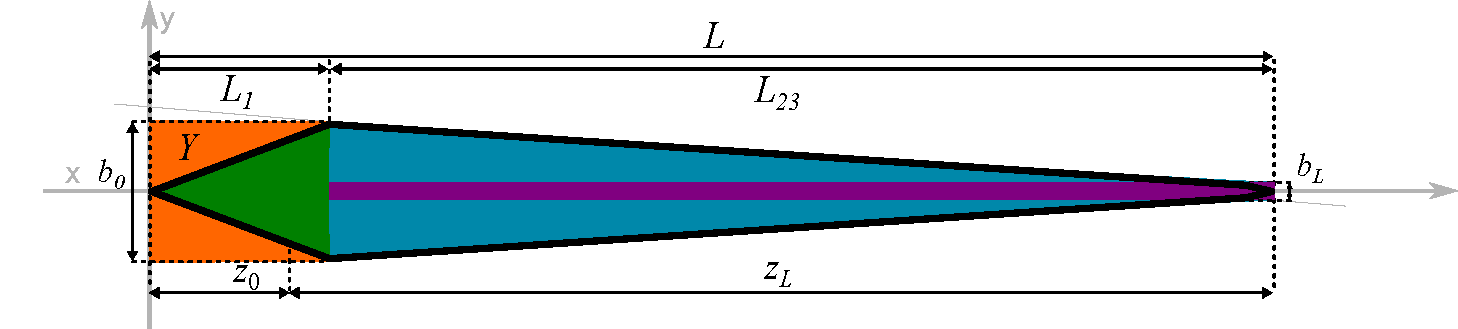
\includegraphics[width=\linewidth]{./images/fffSimplified.pdf}
    \vspace*{-3ex}    
  \end{center}
  \caption[Total area of an AF4 channel in the simplified model]{
    Total area of an AF4 channel in the simplified model.}
  \label{fig:fffSimplied}
\end{figure}
With these assumptions, the channel surface $\AL$ is computed as
\begin{equation}
\AL = \int_{0}^{L} b(z) \diff z 
= 
\intGreenBox{\ensuremath{\frac{1}{2} b_0 L_1}}
+ 
\intPurpleBox{\ensuremath{\bL L_{23}}}
+
\intBlueBox{\ensuremath{\frac{1}{2} \bDelta L_{23}}}
\end{equation}
$Y$ is the enclosed area of the elongation from,
$e_2(x)$ y-axis and $e_1(x)$ and its symmetrical counterpart 
(Fig. \ref{fig:fffApprox1} and \ref{fig:fffApprox2}). 
It can be calculated by simple geometrical considerations (Fig. )as 
\begin{equation}
\intOrangeBox{\ensuremath{Y}} = \intOrangeBox{\ensuremath{ 2 \cdot \frac{1}{2} e_2(0) L_1 }} = 
\intOrangeBox{\ensuremath{ \frac{1}{2}\left( b_0 + \frac{L_1}{L_{23}} \bDelta \right) L_1 }}
\end{equation}

The area, which is relevant for separation, could also be calculated according to the geometrical considerations from 
above.
In this simplified version, the the proximal and distal focusing cases have to be distinguished:
\subsubsection*{Distal focusing with \bm{$z_0  \geqq L_1$}}
In this case, only the relevant part on the elongated surface is considered (Fig. \ref{fig:fffApprox1}).
%\FloatBarrier
\begin{figure}[h]
  \begin{center}
    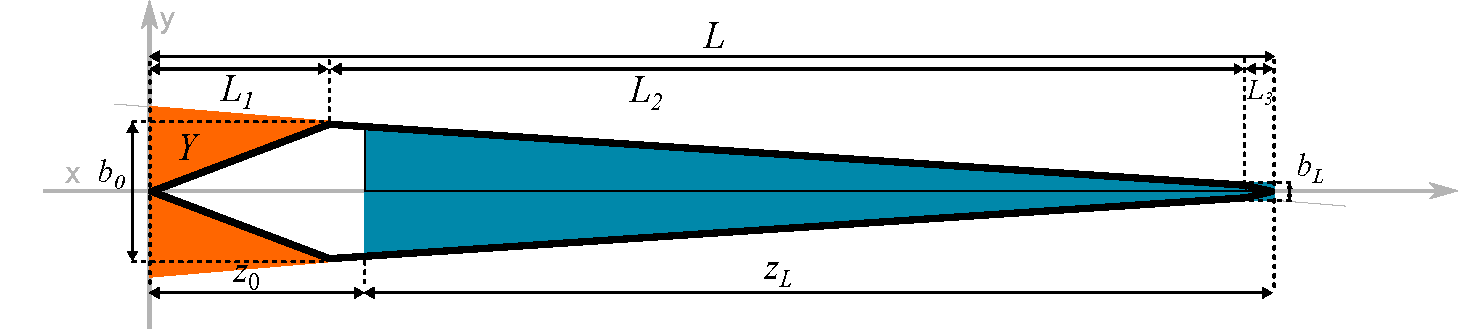
\includegraphics[width=\linewidth]{./images/fffApprox1.pdf}
    \vspace*{-3ex}    
  \end{center}
  \caption[Passed area section - distal focussing, simplified approximation]{
   Simplified model of relevant passed area sections acccording to literature\scite{Litzen1991}  in case of a distal 
   focusing 
   point. }
  \label{fig:fffApprox1} 
\end{figure}
\begin{equation}
\frac{\Vappgeo}{w} = 
 \int_{z_0}^{\zL} b(z) \diff z = 
\frac{1}{2}
%\left( b_0 - b_L  \right)
\bDelta
\left( L_{23} - z_0 \right) 
\end{equation}
\clearpage
\subsubsection*{Proximal focusing with \bm{$z_0 < L_1$}}
In this case, the additional space on the left part has to be considered as well (Fig. \ref{fig:fffApprox2}).
\begin{figure}[H]
  \begin{center}
    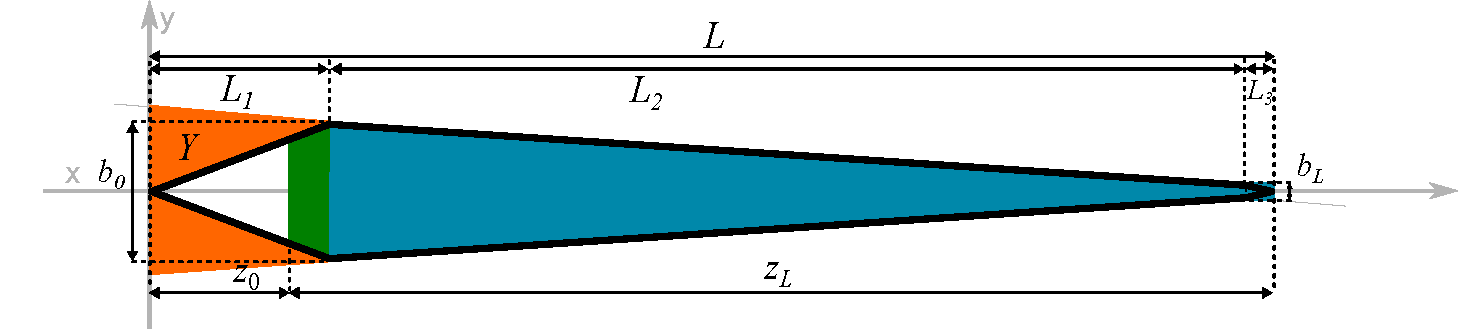
\includegraphics[width=\linewidth]{./images/fffApprox2.pdf}
    \vspace*{-3ex}    
  \end{center}
  \caption[Passed area section - distal focussing, simplified approximation]{
    Simplified model of relevant passed area sections acccording to literature\scite{Litzen1991} 
   in case of a proximal focusing 
    point. }
  \label{fig:fffApprox2}
\end{figure}

\begin{equation}
\frac{\Vappgeo}{w} = 
 \int_{z_0}^{\zL} b(z) \diff z = 
\intGreenBox{ \ensuremath {\frac{b_0}{2 L_1}  (L_1^2-z_0^2) }}
+ \intBlueBox{ \ensuremath { \frac{1}{2} 
    %\left( b_0 - b_L  \right)
    \bDelta
      L_{23} } }
\end{equation}



\section*{Simplified formulation $\bm\whyd$ and Volume $\bm\Vhyd$}
%\section*{Simplified formalism}
A much shorter version has already been derived  with the assumptions $L_{23} = L_2 
+ L_3$ and $b(L) \approx b(L_{12}) = b_L$.\scite{Litzen1991}

Here, 
\begin{equation}
\begin{array}{lll}
\tvoid &= & \frac{\Vappgeo}{\Vc} \ln{
  \left(
  1 + \frac{\Vc}{\Ve}
  \left(
  1 - \frac{
    w 
    \left(
    b_0 z_0 
    - \frac{
      z_0^2 \bDelta
    }{
      2L} 
    - Y
    \right)
  }{\Vgeo}
  \right)
  \right)}
\\\addlinespace
&= &\frac{\Vappgeo}{\Vc} \ln{
  \left(
  1 + \frac{\Vc}{\Ve}
  \left(
  1 - \frac{
    b_0 z_0 
    - \frac{
      z_0^2 \bDelta
    }{
      2L
    } 
    -  Y
  }{
 \int_{0}^{L} b(z) \diff z 
}
  \right)
  \right)}
\end{array}
\end{equation}
\begin{figure}[H]
  \begin{center}
    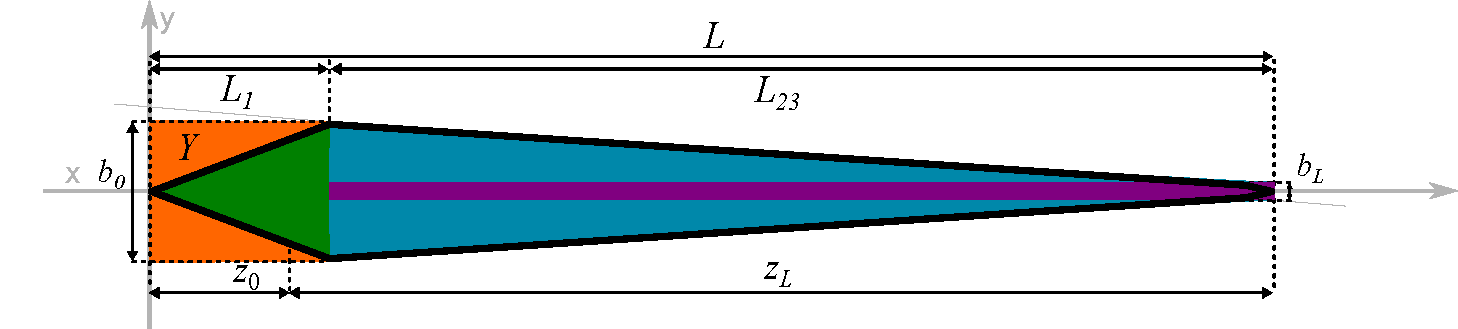
\includegraphics[width=\linewidth]{./images/fffSimplified.pdf}
    \vspace*{-3ex}    
  \end{center}
  \caption[Total area of an AF4 channel in the simplified model]{
    Total area of an AF4 channel in the simplified model.}
  \label{fig:fffSimplied}
\end{figure}
With these assumptions, the channel surface $\AL$ is computed as
\begin{equation}
\AL = \int_{0}^{L} b(z) \diff z 
= 
\intGreenBox{\ensuremath{\frac{1}{2} b_0 L_1}}
+ 
\intPurpleBox{\ensuremath{\bL L_{23}}}
+
\intBlueBox{\ensuremath{\frac{1}{2} \bDelta L_{23}}}
\end{equation}
$Y$ is the enclosed area of the elongation from,
$e_2(x)$ y-axis and $e_1(x)$ and its symmetrical counterpart 
(Fig. \ref{fig:fffApprox1} and \ref{fig:fffApprox2}). 
It can be calculated by simple geometrical considerations (Fig. \ref{fig:fffSimplied}) as 
\begin{equation}
\intOrangeBox{\ensuremath{Y}} = \intOrangeBox{\ensuremath{ 2 \cdot \frac{1}{2} e_2(0) L_1 }} = 
\intOrangeBox{\ensuremath{ \frac{1}{2}\left( b_0 + \frac{L_1}{L_{23}} \bDelta \right) L_1 }}
\end{equation}

The area, which is relevant for separation, could also be calculated according to the geometrical considerations from 
above.
In this simplified version, the the proximal and distal focusing cases have to be distinguished:
\subsubsection*{Distal focusing with \bm{$z_0  \geqq L_1$}}
In this case, only the relevant part on the elongated surface is considered (Fig. \ref{fig:fffApprox1}).
%\FloatBarrier
\begin{figure}[h]
  \begin{center}
    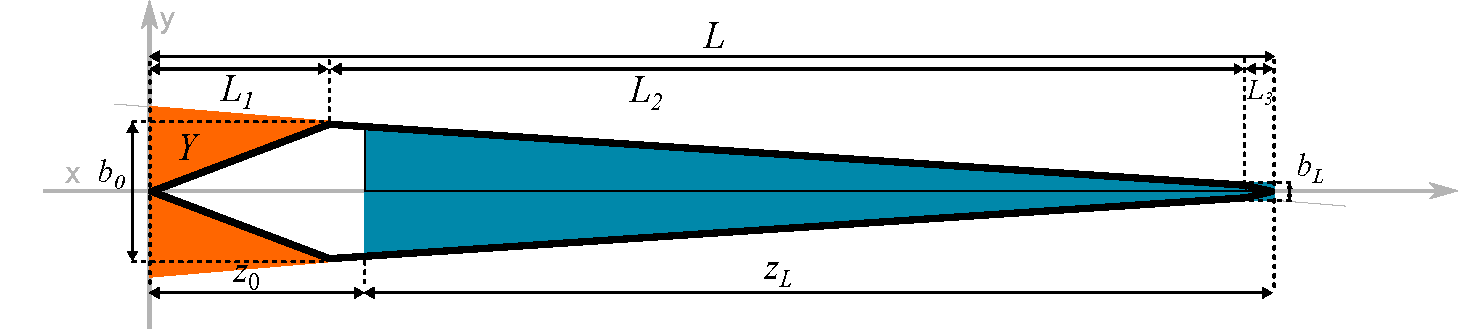
\includegraphics[width=\linewidth]{./images/fffApprox1.pdf}
    \vspace*{-3ex}    
  \end{center}
  \caption[Passed area section - distal focussing, simplified approximation]{
   Simplified model of relevant passed area sections acccording to literature\scite{Litzen1991}  in case of a distal 
   focusing 
   point. }
  \label{fig:fffApprox1} 
\end{figure}
\begin{equation}
\frac{\Vappgeo}{w} = 
 \int_{z_0}^{\zL} b(z) \diff z = 
\frac{1}{2}
%\left( b_0 - b_L  \right)
\bDelta
\left( L_{23} - z_0 \right) 
\end{equation}
\FloatBarrier
\subsubsection*{Proximal focusing with \bm{$z_0 < L_1$}}
In this case, the additional space on the left part has to be considered as well (Fig. \ref{fig:fffApprox2}).
\begin{figure}[H]
  \begin{center}
    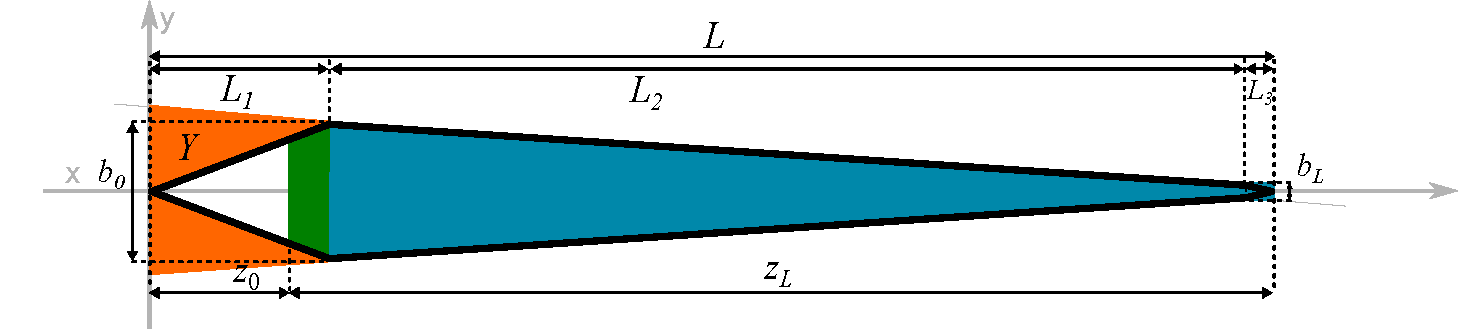
\includegraphics[width=\linewidth]{./images/fffApprox2.pdf}
    \vspace*{-3ex}    
  \end{center}
  \caption[Passed area section - distal focussing, simplified approximation]{
    Simplified model of relevant passed area sections acccording to literature\scite{Litzen1991} 
   in case of a proximal focusing 
    point.}
  \label{fig:fffApprox2}
\end{figure}

\begin{equation}
\frac{\Vappgeo}{w} = 
 \int_{z_0}^{\zL} b(z) \diff z = 
\intGreenBox{ \ensuremath {\frac{b_0}{2 L_1}  (L_1^2-z_0^2) }}
+ \intBlueBox{ \ensuremath { \frac{1}{2} 
    %\left( b_0 - b_L  \right)
    \bDelta
      L_{23} } }
\end{equation}



\section*{Determination of without experimental $\tvoid$}
If a calibration measurement with known diffusion coefficient is used the relationship of $R$ can be formulated as used 
as well. $R_D$ stands for the dependency of $R$ the calibration
\begin{equation}
R_D(w) = 6\lambda \left( \coth{\left( \frac{1}{2\lambda} \right) } - 2\lambda \right)
\end{equation}

\begin{equation}
\lambda = \frac{D V}{\Vc w^2} = \frac{D \AL}{\Vc w}
\end{equation}

In order to eliminate $\tvoid$ as experimental input, eq. \ref{eq:CFEquation} is used as a substitution for the 
retention ratio, resulting in an expression solely dependent on $\te$ and $w$:
\begin{equation}
R_{\te}(w) = \frac{2 \CF w}{\te}
\end{equation}
By adjusting $w$ such that \[\left( R_{\te} - R_D \right)^2 \rightarrow \min\]
$w$ can be calculated. This corresponds (as an exact solution) to the literature to the "calibration method 5", 
presented by Wahlund \scite{Wahlund2013} and remains as the only recommended calibration method according to the 
results presented in the main paper.


\section*{UML class diagram}
Perhaps, but not mandatory

\section*{User interface}

2 images 
\clearpage
\section*{Detailed description of applied algorithms}
\subsection*{Classical Calibration}

\subsubsection*{Inputs:}
\begin{multicols}{3}
  \begin{packed_item}
  \item void peak $\tvoid$
  \item elution flow $\Ve$
  \item elution time $\te$
  \item cross flow $\Vc$
  \item \small diffusion coefficient \normalsize $D$
  \item relative focus $\zP$;
   % \item channelLength $L$
  \end{packed_item}
\end{multicols}

\subsubsection*{Outputs:}
\begin{multicols}{3}
  \begin{packed_item}
  \item channel width $w$
    % \item volume $V^{hyd}$
  \item channel volume $V^0$
  \end{packed_item}
\end{multicols}

\subsubsection*{Constants:}
\begin{multicols}{3}
  \begin{packed_item}
    % \item volume $V^0$
    \item $\wmin \leftarrow 10^{-4}$
    \item  $\wmax \leftarrow 10$
  \end{packed_item}
\end{multicols}

\subsubsection*{Temporary variables:}
\begin{multicols}{3}
  \begin{packed_item}
    % \item volume $V^0$
  \item measured\enspace retention $\Rmeas$
  \item variation $δ_w$
  \item $\lambda$
  \end{packed_item}
\end{multicols}

\subsubsection*{Calculations:}

\subparagraph{1}
Calculate volume:

      %       \[ \Vgeo \leftarrow \frac{\Vc \cdot \tvoid}{ \ln{ \left( \dfrac{ \zP  - \nicefrac{(\Ve + \Vc)}{\Vc}      }{ 1 - \nicefrac{(\Ve + \Vc)}{\Vc}          } \right) }} \]

\begin{algorithmic}
  \State  \[V^0 \leftarrow \frac{V_c \cdot \tvoid}{ \ln{ \left( \dfrac{ z_\% - \nicefrac{(V_e + V_c)}{V_c}      }{ 1 - 
  \nicefrac{(V_E + V_c)}{V_c}          } \right) }} \]
\end{algorithmic}

\subparagraph{2}
Calculate \Rmeas:
\begin{algorithmic}
  \State  \[ \Rmeas \leftarrow \frac{\tvoid}{\te} \]
\end{algorithmic}
\subparagraph{3}
Initialize $w$ and $δ$:
\[ w \leftarrow \frac{\wmax + \wmin}{2} \]
\[ δ_w \leftarrow \frac{\wmax - \wmin}{4} \]
\clearpage
\subparagraph{4}
Find $w$ such that $|\Rmeas - \Rcalc| \stackrel{!}{=}\text{min}$ by bisection:
\begin{algorithmic}
  \For{$i \leftarrow 0$ to $50$}
  \State $\lambda \leftarrow  \frac{D \cdot V^0}{V_C \cdot w^2}$     
  \State $ \Rcalc \leftarrow 6 \lambda \left(\frac{1}{\tanh(1 / 2 \lambda)} - 2 \lambda \right)$  \# $\nicefrac{1}{\tanh{(x)}} = \coth(x) $
  \If{$ \Rcalc > \Rmeas$}
  \State  $w \leftarrow w + δ_w$
  \Else
  \State $w \leftarrow w - δ_w$
  \EndIf
  \State $δ_w \leftarrow δ_w / 2$
  \EndFor
\end{algorithmic}
\clearpage
%%%%%%%%%%%%%%%%%%%%%%%%%%%%%%%%%%%%%%%%%%%%%%%%%%%%%%%%%%%%%%%%%%%%%%%%%%%%%%%%%%%%%%%%%%%%%%%%%%%%
%%%
%%%%%%%%%%%%%%%%%%%%%%%%%%%%%%%%%%%%%%%%%%%%%%%%%%%%%%%%%%%%%%%%%%%%%%%%%%%%%%%%%%%%%%%%%%%%%%%%%%%%
\subsection*{Classical Calibration under consideration of the simpiflied trapezoidal
shape model}

\subsubsection*{Inputs:}
\begin{multicols}{3}
  \begin{packed_item}
    \item void peak $\tvoid$
    \item elution flow $\Ve$
    \item elution time $\te$
    \item cross flow $\Vc$
    \item \small diffusion coefficient \normalsize $D$
    \item relative focus $\zP$;
    \item $L_1, L_2, L_3$
    \item $b_0, \bL$
    % \item channelLength $L$
  \end{packed_item}
\end{multicols}

\subsubsection*{Outputs:}
\begin{multicols}{3}
  \begin{packed_item}
    \item channel width $w$
    % \item volume $V^{hyd}$
    \item channel volume $\Vappgeo$
  \end{packed_item}
\end{multicols}

\subsubsection*{Constants:}
\begin{multicols}{3}
  \begin{packed_item}
    % \item volume $V^0$
    \item $\wmin \leftarrow 10^{-4}$
    \item  $\wmax \leftarrow 10$
  \end{packed_item}
\end{multicols}

\subsubsection*{Temporary variables:}
\begin{multicols}{3}
  \begin{packed_item}
    % \item volume $V^0$
    \item measured\enspace retention $\Rmeas$
    \item Channel surface area $\AL$
%    \item variation $δ_w$
    \item $\lambda$
    \item $\tmp1$
  \end{packed_item}
\end{multicols}

\subsubsection*{Calculations:}

\subparagraph{1}
Calculate volume:

%       \[ \Vgeo \leftarrow \frac{\Vc \cdot \tvoid}{ \ln{ \left( \dfrac{ \zP  - \nicefrac{(\Ve + \Vc)}{\Vc}      }{ 1 - 
%\nicefrac{(\Ve + \Vc)}{\Vc}          } \right) }} \]

\begin{algorithmic}
  \State $L_{23} \leftarrow L_2 + L_3$,\qquad $\bDelta \leftarrow b_0 - \bL$
  \State $\AL \leftarrow \frac{1}{2} b_0 L_1 + b_L L_{23} + \frac{1}{2} \bDelta L_{23}$
  \State $ Y \leftarrow \frac{1}{2} \left( b_0 +\frac{L_1}{L_{23}} \right) L_1$
  \State $\tmp1 \leftarrow b_0 z_0 
  - \frac{ z_0^2 \bDelta  }{  2L} - Y $
  %%%% Alternative calculation for 1-A(z) instead of AL
%  \If {$z_0 \geqq L_1$}
%  \State $\tmp1 \leftarrow \frac{ \tmp1}{ 
%    \frac{1}{2} 
%  \bDelta
%    \left( L_{23} - z_0 \right)
%  } $
%  \Else 
%  \State $\tmp1 \leftarrow \frac{ \tmp1}{ 
%    \frac{b_0}{2L_1}\left( L_1^2 - z_0^2 \right)
%    + \frac{1}{2} \bDelta L_23  
%  } $
%  \EndIf
  \State $\tmp1 \leftarrow 1 - \frac{\tmp1}{\AL} $
  \State $\tmp1 \leftarrow \ln{\left( 1 + \frac{\Vc}{\Ve} \tmp1 \right)}$
  \State $\Vappgeo \leftarrow \frac{\Vc\tvoid}{\tmp1}$
\end{algorithmic}

\subparagraph{2}
Calculate \Rmeas:
\begin{algorithmic}
  \State  \[ \Rmeas \leftarrow \frac{\tvoid}{\te} \]
\end{algorithmic}
\subparagraph{3}
Initialize $w$ and $δ$:
\[ w \leftarrow \frac{\wmax + \wmin}{2} \]
\[ δ_w \leftarrow \frac{\wmax - \wmin}{4} \]
\clearpage
\subparagraph{4}
Find $w$ such that $|\Rmeas - \Rcalc| \stackrel{!}{=}\text{min}$ by bisection:
\begin{algorithmic}
  \For{$i \leftarrow 0$ to $50$}
  \State $\lambda \leftarrow  \frac{D \cdot \Vappgeo}{V_C \cdot w^2}$     
  \State $ \Rcalc \leftarrow 6 \lambda \left(\frac{1}{\tanh(1 / 2 \lambda)} - 2 \lambda \right)$  \# 
  $\nicefrac{1}{\tanh{(x)}} = \coth(x) $
  \If{$ \Rcalc > \Rmeas$}
  \State  $w \leftarrow w + δ_w$
  \Else
  \State $w \leftarrow w - δ_w$
  \EndIf
  \State $δ_w \leftarrow δ_w / 2$
  \EndFor
\end{algorithmic}
\clearpage
%%%%%%%%%%%%%%%%%%%%%%%%%%%%%%%%%%%%%%%%%%%%%%%%%%%%%%%%%%%%%%%%%%%%%%%%%%%%%%%%%%%%%%%%%%%%%%%%%%%%
%%%
%%%%%%%%%%%%%%%%%%%%%%%%%%%%%%%%%%%%%%%%%%%%%%%%%%%%%%%%%%%%%%%%%%%%%%%%%%%%%%%%%%%%%%%%%%%%%%%%%%%%
\subsection*{Calibration of channel height by $\bm{V^{\text{geo}}}$}
\newcommand{\lamMin}{\ensuremath{\lambda_\text{min}}}
\newcommand{\lamMax}{\ensuremath{\lambda_\text{max}}}
\subsubsection*{Inputs:}
\begin{multicols}{3}
  \begin{packed_item}
    \item void peak $\tvoid$
%    \item elution flow $\Ve$ 
    \item elution time $\te$
    \item cross flow $\Vc$
    \item \small diffusion coefficient \normalsize $D$
    \item relative focus $\zP$;
    \item $L_1, L_2, L_3$
    \item $b_0, \bL$
    % \item channelLength $L$
  \end{packed_item}
\end{multicols}

\subsubsection*{Outputs:}
\begin{multicols}{3}
  \begin{packed_item}
    \item channel height $w$ 
    \item channel volume $\Vgeo$    
  \end{packed_item}
\end{multicols}

\subsubsection*{Temporary variables:}
\begin{multicols}{3}
  \begin{packed_item}
    % \item volume $V^0$
    \item measured\enspace retention $\Rmeas$
    \item calculated\enspace retention $\Rcalc$
    \item variation $δ_λ$
    \item $λ$
    \item $S$
    \item $L_{12}, L$
    \item $z_0$
    \item $m_1, m_2$
    \item $t_2$
%    \item $A_z$
    \item $\AL$
    \item $A_3$
  \end{packed_item}
\end{multicols}

\subsubsection*{Constants:}
\begin{multicols}{3}
  \begin{packed_item}
    \item $\lamMin \leftarrow 10^{-5}$
    \item  $\lamMax \leftarrow 100$ 
    \end{packed_item}
  \end{multicols}
\subsubsection*{Calculations:}

\subparagraph{1}
Calculate $\Rmeas$:\vspace*{-4ex}
\begin{algorithmic}
  \State  \[ \Rmeas \leftarrow \frac{\tvoid}{\te} \]
\end{algorithmic}

\subparagraph{2}
Initialize $λ$ and $δ_λ$:\vspace*{-4ex}
\[ λ \leftarrow \frac{\lamMin + \lamMax}{2} \]\vspace*{-1.55ex}
\[ δ_λ \leftarrow \frac{\lamMax - \lamMin}{4} \]
\vspace*{-1ex}
\subparagraph{3}
Find $λ$ such that $|\Rmeas - \Rcalc| \stackrel{!}{=}\text{min}$ by bisection:
\begin{spacing}{1.1}
\begin{algorithmic}
  \For{$i \leftarrow 0$ to $50$}
  \State $ \Rcalc \leftarrow 6 \lambda \left(\frac{1}{\tanh(1 / 2 \lambda)} - 2 \lambda \right)$  \# 
  $\nicefrac{1}{\tanh{(x)}} = \coth(x) $
  \If{$ \Rcalc > \Rmeas$}
  \State  $λ \leftarrow λ + δ_λ$
  \Else
  \State $λ \leftarrow λ - δ_λ$
  \EndIf
  \State $δ_λ \leftarrow δ_λ / 2$
  \EndFor
\end{algorithmic}
\end{spacing}
\vspace*{-2ex}
\subparagraph{4}
Calculate substitution term $S$:\vspace*{-7.5ex}
\begin{algorithmic}
  \State  \[ S \leftarrow \ddfrac{λ \cdot \Vc }{D} \]
\end{algorithmic}\vspace*{-3.5ex}
\begin{comment}
\subparagraph{5} Calculate passed channel area $A_z$:
\begin{algorithmic}
  \State $\displaystyle A_3 \leftarrow \frac{1}{2}\cdot \bL L_3
   \qquad L_{12} \leftarrow L_1 + L_2 
   \qquad L \leftarrow L_{12} + L_3 
   \qquad z_0 \leftarrow z_\% \cdot L $\vspace*{.5ex}
  \If{$ z_0 \geqq L_1$}
  \State $\displaystyle m_2 \leftarrow \frac{b_0 - \bL}{2\cdot L_2}
           \qquad \bDelta \leftarrow b_0 - \bL
           \qquad t_2 \leftarrow \frac{1}{2}\left(b_0 + \frac{L_1}{L_2} \bDelta \right) 
           $\vspace*{.5ex}
  \State  $ A_z \leftarrow (L_{12} - z_0)\cdot( m_2  (L_{12} + z_0) + t_2 ) +  A_3$
  \Else
  \State $m_1 \leftarrow \frac{b_0}{2 L_1}$
  \State  $ A_z \leftarrow  m_1 \cdot (L_1^2 - z_0^2) + \frac{1}{2}(b_0 + b_L)L_2  + A_3 $
  \EndIf
\end{algorithmic}
\end{comment}
\subparagraph{5} Calculate membrane area $\AL$:
\begin{algorithmic}
  \State $       A_1 \leftarrow \frac{1}{2} b_0  L_1  
  \qquad A_2 \leftarrow  \frac{1}{2} (b_0 + b_L) L_2  
  \qquad A_3 \leftarrow \frac{1}{2} L_3\bL  
  $\vspace*{.5ex}
  \State $  \AL \leftarrow A_1 + A_2 + A_3
  $\vspace*{.5ex}
\end{algorithmic}

\subparagraph{6} Calculate $w$:\vspace*{-6.5ex}
\begin{algorithmic}
  \State  \[ w \leftarrow \ddfrac{\AL}{S} \]
\end{algorithmic}

\subparagraph{7} Calculate $\Vgeo$:\vspace*{-6.5ex}
\begin{algorithmic}
  \State  \[ \Vgeo \leftarrow \AL \cdot w \]
\end{algorithmic}
\clearpage
%%%%%%%%%%%%%%%%%%%%%%%%%%%%%%%%%%%%%%%%
%%%
%%%
%%%%%%%%%%%%%%%%%%%%%%%%%%%%%%%%%%%%%%%%
\subsection*{Calibration of channel height by $\bm{\Vhyd}$}
\subsubsection*{Inputs:}
\label{sec:CalibVhyd}
\begin{multicols}{3}
  \begin{packed_item}
    \item void peak \tvoid
    \item elution flow \Ve
%    \item elution time $\te$
    \item cross flow \Vc
%    \item \small diffusion coefficient \normalsize $D$
    \item relative focus \zP;
    \item $L_1, L_2, L_3$
    \item $b_0$, \bL
    % \item channelLength $L$
  \end{packed_item}
\end{multicols}

\subsubsection*{Outputs:}
\begin{multicols}{3}
  \begin{packed_item}
    \item channel width $w$
    \item channel volume $\Vhyd$
  \end{packed_item}
\end{multicols}

\subsubsection*{Temporary variables:}
%\newcommand{\vartmp}[1]{\ensuremath{\text{tmp}_{#1}}}
\begin{multicols}{3}
  \begin{packed_item}
  \item $z_0$
  \item $\Vin$
  \item $L_{12}, L$  
  \item $\bDelta$
  \item $m_1, m_2, m_3$
  \item $t_2, t_3$
 % \item $α_2, α_3$
 % \item $β_1, β_2, β_3$
  %\item $γ_2, γ_3$
 % \item $δ_1, δ_2, δ_3$
%  \item $Δ_2, Δ_3$
  \item $\CFone, \CFtwo, \CFthree, \CF$
 \item $\tmp1, \tmp2$
  \end{packed_item}
\end{multicols}
\subsubsection*{Calculations:}
\subparagraph{1}
Calculate "derived" parameters:
\begin{algorithmic}
\State $L_{12} \leftarrow L_1 + L_2
        \qquad L \leftarrow L_{12} + L_3
        \qquad z_0 \leftarrow \zP \cdot L
        \qquad \bDelta \leftarrow  b_0 - \bL
        \qquad \Vin \leftarrow \Ve + \Vc
        $
\end{algorithmic}
\subparagraph{2}
Calculate slopes and offsets of the border lines of the channel plain:
\begin{algorithmic}
  \State $       m_1 \leftarrow   \frac{b_0}{2L_1}
          \qquad m_2 \leftarrow - \frac{\bDelta}{2L_2}
          \qquad m_3 \leftarrow - \frac{\bL}{2L_3}
         $\vspace*{.5ex}
  \State $           t_2 \leftarrow \frac{1}{2} \left( b_0 +  \frac{L_1}{L_2}\bDelta \right)
              \qquad t_3 \leftarrow \frac{L \bL}{2 L_3 }
         $\vspace*{.5ex}
\end{algorithmic}
\subparagraph{3}
Calculate area sections of the channel plain:
\begin{algorithmic}
  \State $       A_1 \leftarrow \frac{1}{2} b_0  L_1  
          \qquad A_2 \leftarrow  \frac{1}{2} (b_0 + b_L) L_2  
          \qquad A_3 \leftarrow \frac{1}{2} L_3\bL  
         $\vspace*{.5ex}
  \State $  \AL \leftarrow A_1 + A_2 + A_3
  $\vspace*{.5ex}
\end{algorithmic}

\begin{comment}

%%%%
% The analytical solution is omitted and substituted by the numerical procedure below
%%%


\subparagraph{4}



Calculate substitution parameters and discriminants:\\\textbf{}
$ \begin{array}{llll}
  &α_2 \leftarrow \frac{t_2}{m_2}
  &α_3 \leftarrow \frac{t_3}{m_3}
  \\\addlinespace[.75ex]
  %\State $   
  β_1 \leftarrow -\frac{\Vc m_1}{ \AL }
  &β_2 \leftarrow -\frac{\Vc m_2}{ \AL }
  &β_3 \leftarrow -\frac{\Vc m_3}{ \AL }
      \\\addlinespace[.75ex]
  %\State $   
  &γ_2 \leftarrow -\frac{2 \Vc t_2}{\AL}
  &γ_3 \leftarrow -\frac{2 \Vc t_3}{\AL}
      \\\addlinespace[.75ex]
  δ_1 \leftarrow \Vin
  &\multicolumn{2}{l}{δ_2 \leftarrow \Vin - \frac{\Vc}{\AL} \left( A_1 - m_2L_1^2 - 2t_2L_1  \right)}
  &\\
  &\multicolumn{2}{l}{δ_3 \leftarrow \Vin - \frac{\Vc}{\AL} \left( A_1 + A_2 - m_3L_{12}^2 - 2t_3L_{12} \right) }
    \\\addlinespace[.75ex]
%  \State $   
  &Δ_2 \leftarrow 4β_2 δ_2 - γ_2^2
  &Δ_3 \leftarrow 4β_3 δ_3 - γ_3^2
  \end{array} $\clearpage
\subparagraph{5}
Calculate conversion factor \CF:
\begin{algorithmic}
    \If{$ Δ_3 > 0 $}
      \State $ \CFthree \leftarrow \text{IntPosDisc}\left( α_3,β_3,γ_3,δ_3,Δ_3,L_{12},L,m_3 \right)$
    \Else
     \State $ \CFthree \leftarrow \text{IntNegDisc}\left( α_3,β_3,γ_3,δ_3,Δ_3,L_{12},L,m_3 \right)$
    \EndIf\vspace*{1.5ex}
  \If{$z_0 \geqq L_1$}
    \If{$ Δ_2 > 0 $}
      \State $ \CFtwo \leftarrow \text{IntPosDisc}\left( α_2,β_2,γ_2,δ_2,Δ_2,z_0,L_{12},m_2 \right)$
    \Else
      \State $ \CFtwo \leftarrow \text{IntNegDisc}\left( α_2,β_2,γ_2,δ_2,Δ_2,z_0,L_{12},m_2 \right)$
    \EndIf
    \State $\CF \leftarrow \CFtwo + \CFthree$
  \Else    
    \If{$ Δ_2 > 0 $}    
      \State $ \CFtwo \leftarrow \text{IntPosDisc}\left( α_2,β_2,γ_2,δ_2,Δ_2,L_1,L_{12},m_2 \right)$
    \Else
      \State $ \CFtwo \leftarrow \text{IntNegDisc}\left( α_2,β_2,γ_2,δ_2,Δ_2,L_1,L_{12},m_2 \right)$
    \EndIf
      \State $\CFone \leftarrow \text{IntOne}\left( β_1,δ_1,z_0,L_1,m_1 \right)$
    \State $\CF \leftarrow \CFone + \CFtwo + \CFthree$
  \EndIf
\end{algorithmic}

\end{comment}

\subparagraph{4}
Simple numerical integration via Riemann sum (see subroutines):
\begin{algorithmic}
  \State $\CF \leftarrow \text{calcCF}(.....)$
\end{algorithmic}
\subparagraph{5}
Calculate $w$:
\begin{algorithmic}
\State $w \leftarrow \ddfrac{\tvoid}{2\cdot\CF} $
\end{algorithmic}
\begin{comment}
\subparagraph{7}
Calculate passed channel area $A$:
\begin{algorithmic}
  \If{$ z_0 \geqq L_1$}
\State  $ A_z \leftarrow (L_{12} - z_0)\cdot( m_2  (L_{12} + z_0) + t_2 ) +  A_3$
\Else
\State  $ A_z \leftarrow  m_1 \cdot (L_1^2 - z_0^2) + A_2 + A_3 $
\EndIf
\end{algorithmic}
\end{comment}

\subparagraph{6}
Calculate $\Vhyd$ with passed area:
\begin{algorithmic}
  \State $\Vhyd \leftarrow A_\xi \cdot w$
\end{algorithmic}
\clearpage
\subsubsection*{S\quad subroutines}
\vspace*{-1.2ex}
\subparagraph{S1} calcCF
\vspace*{-1.2ex}
\begin{algorithmic}
  \State \tiny \# initialize \xi near $z_0$ on the \xi-grid \normalsize
  \State $\Delta\xi \leftarrow \frac{L}{n}$
  \State $\xi < z_0$
  \While{ $\xi < z_0$ }
  \State $\xi \leftarrow \xi + \Delta\xi$
  \EndWhile
  \State \tiny \# Calculate $\CFone$ \normalsize
  \While{ $\xi < z_0$ }
  \State  $A_\xi \leftarrow m_1 \xi^2 $
  \State $ \Vxi \leftarrow \Vin - \Vc \frac{A_\xi}{\AL} $ 
  \State $E_{\dot{V}\xi} \leftarrow \frac{m_1\xi}{\Vxi} $
  \State $\CF1 \leftarrow \CF1 + E_{\dot{V}\xi} \Delta\xi$
  \State $\xi \leftarrow \xi + \Delta\xi$
  \EndWhile
  \State \tiny \#  Calculate $\CFtwo$ \normalsize
  \While{ $\xi < L_{12}$ }
  \State $A_\xi \leftarrow A_1 + m_2 \left( \xi^2 - L_1^2 \right) + 2 t_2\left(\xi - L_1\right) $
  \State $ \Vxi \leftarrow \Vin - \Vc \frac{A_\xi}{\AL} $ 
  \State $E_{\dot{V}\xi} \leftarrow \frac{m_2\xi + t_2}{\Vxi} $
  \State $\CF2 \leftarrow \CF2 + E_{\dot{V}\xi} \Delta\xi$
  \State $\xi \leftarrow \xi + \Delta\xi$
  \EndWhile
  \State \tiny \#  Calculate $\CFthree$ \normalsize
  \While{ $\xi < L$ }
  \State $A_\xi \leftarrow A_1 + A_2 + m_3 \left( \xi^2 - L_{12}^2 \right) + 2 t_3\left(\xi - L_{12}\right) $
  \State $ \Vxi \leftarrow \Vin - \Vc \frac{A_\xi}{\AL} $ 
  \State $E_{\dot{V}\xi} \leftarrow \frac{m_3\xi + t_3}{\Vxi} $
  \State $\CF3 \leftarrow \CF3 + E_{\dot{V}\xi} \Delta\xi $
  \State $\xi \leftarrow \xi + \Delta\xi $
  \EndWhile
\end{algorithmic}
\vspace*{-2.0ex}
\subsubsection*{General formulation of numerical $\boldsymbol{C_\text{F}}$ integration for arbitrary 
  channel shapes}
\vspace*{-.5ex}
The simple integration procedure above for three channel sections could also be generalized by the following when the 
channel shape is provided as a set of functions $e_s(x)$:
%% optimal shapes \scite{CarinasDiss, Wahlund etc. }
\begin{algorithmic}
  \For{$s \leftarrow 1 $ to $S$}
  \While{ $\xi < L$ }
  \State $A_\xi \leftarrow \displaystyle\sum_{\sigma=1}^{s}A_\sigma + \displaystyle\int_{L1s}^\xi e_s(x) \diff x $
  \State $ \Vxi \leftarrow \Vin - \Vc \frac{A_\xi}{\AL} $ 
  \State $E_{\dot{V}\xi} \leftarrow \frac{e_s(\xi)}{\Vxi} $
  \State $\CF \leftarrow \CF + E_{\dot{V}\xi} \Delta\xi $
  \State $\xi \leftarrow \xi + \Delta\xi $
  \EndWhile
  \EndFor
\end{algorithmic}
\vspace*{-0.5ex}
Alternatively, the Riemann sum could be exchanged by a trapezoidal rule approach.
\needspace{30em}
\begin{comment} 
%%%%%%%%%%%%
%% Removed as this is better done numerically
%%%%%%%%%%%%
\subparagraph{S1}
Polynomial $P$:
\begin{algorithmic}
\State $P(β,γ,δ,ξ) \coloneqq βξ^2+γξ+δ$
\end{algorithmic}
\subparagraph{S2}\textbf{}
\begin{algorithmic}
  \State $\text{IntPosDisc}(α,β,γ,δ,Δ,s_0,s_1,m_i) \coloneqq$\vspace*{1ex}
  \State $\CFi  \leftarrow \ln(\frac{P(β, γ, δ, s_1) }{  P(β, γ, δ, s_0)})$\vspace*{1ex}
  \State $\CFi  \leftarrow \frac{\CFi}{2β} $\vspace*{1ex}
  \State $\tmp0 \leftarrow \sqrt{Δ}$\vspace*{1ex}
  \State $\tmp1 \leftarrow \text{arctan}\left(\frac{2βs_1+γ}{\tmp0} \right) $\vspace*{1ex}
  \State $\tmp2 \leftarrow \text{arctan}\left(\frac{2βs_0+γ}{\tmp0} \right)$\vspace*{1ex}
  \State $\tmp3 \leftarrow \left(\frac{2}{\tmp0} \right)\cdot \left( α - \frac{γ}{β} \right) \cdot 
  \left(\tmp1-\tmp2\right) $\vspace*{1ex}
  \State $\CFi \leftarrow \left( \CFi + \tmp3 \right)  \cdot m_i $\vspace*{1ex}
  \State \Return \CFi
\end{algorithmic}
\subparagraph{S3}
\begin{algorithmic}
  \State $\text{IntNegDisc}(α,β,γ,δ,Δ,s_0,s_1,m_i) \coloneqq $  \vspace*{1ex}
  \State $\CFi \leftarrow \ln(\frac{P(β, γ, δ, s_1) }{  P(β, γ, δ, s_0)})$\vspace*{1ex}
  \State $\CFi \leftarrow \frac{\CFi}{2β} $\vspace*{1ex}
  \State $\tmp0 \leftarrow \sqrt{-Δ}$ \vspace*{1ex}
  \State $\tmp1 \leftarrow \left( 2 \cdot β \cdot s_1 + γ \right)\left( 2 \cdot β \cdot s_0 + γ \right) $ \vspace*{1ex}
  \State $\tmp1 \leftarrow \tmp0 - \frac{\tmp1}{\tmp0}  $ \vspace*{1ex}
  \State $\tmp1 \leftarrow \frac{2 \cdot β \cdot (s_1 - s_0)}{\tmp1} $ \vspace*{1ex}
  \State $\tmp1 \leftarrow \text{artanh}(\tmp1)$ \vspace*{1ex}
  \State $\tmp1 \leftarrow \left(\frac{2}{\tmp0} \right)\cdot \left( α - \frac{γ}{β} \right) \cdot \tmp1 $
  \vspace*{1ex}
  \State $\CFi \leftarrow \left( \CFi - \tmp1 \right) \cdot m_i $  \vspace*{1ex}
  \State \Return \CFi
\end{algorithmic}
\subparagraph{S4}
\begin{algorithmic}
  \State $\text{IntOne}(β,δ,s_0,s_1,m_1) \coloneqq $  \vspace*{1ex}
  \State $\tmp0 \leftarrow \frac{δ}{β}$
  \State $ \CFone \leftarrow \ln \left| \tmp0 +  s_1^2\right| $
  \State $ \CFone \leftarrow \CFone - \ln \left| \tmp0 +  s_0^2\right| $
  \State $ \CFone \leftarrow \frac{m_1}{2 β} \cdot \CFone $

  \State \Return \CFone
\end{algorithmic}
%\subparagraph{S2}
%\begin{algorithmic}
%\State $\text{Delta}(β,γ,δ) \coloneqq 4βδ-γ^2$
%\end{algorithmic}
\clearpage
%xxxxxxxxxxxxxxxxxxxxxxxxxx
\end{comment}
\clearpage
\subsection*{Calibration of channel height by $\bm{\VnoTvoid}$}
\subsubsection*{Inputs:}
\label{sec:CalibVhyd}
\begin{multicols}{3}
  \begin{packed_item}
    \item void peak \tvoid
    \item elution flow \Ve
    %    \item elution time $\te$
    \item cross flow \Vc
    %    \item \small diffusion coefficient \normalsize $D$
    \item relative focus \zP;
    \item $L_1, L_2, L_3$
    \item $b_0$, \bL
    % \item channelLength $L$
  \end{packed_item}
\end{multicols}

\subsubsection*{Outputs:}
\begin{multicols}{3}
  \begin{packed_item}
    \item channel width $w$
    \item channel volume $\VnoTvoid$
  \end{packed_item}
\end{multicols}

\subsubsection*{Temporary variables:}
%\newcommand{\vartmp}[1]{\ensuremath{\text{tmp}_{#1}}}
\begin{multicols}{3}
  \begin{packed_item}
    \item $z_0$
    \item $\Vin$
    \item $L_{12}, L$  
    \item $\bDelta$
    \item $m_1, m_2, m_3$
    \item $t_2, t_3$
    %\item $α_2, α_3$
    %\item $β_1, β_2, β_3$
   % \item $γ_2, γ_3$
  %  \item $δ_1, δ_2, δ_3$
%    \item $Δ_2, Δ_3$
    \item $\CFone, \CFtwo, \CFthree, \CF$
 %   \item $\tmp1, \tmp2$
  \end{packed_item}
\end{multicols}
\subsubsection*{Calculations:}
\subparagraph{1}
Calculate "derived" parameters:
\begin{algorithmic}
  \State $L_{12} \leftarrow L_1 + L_2
  \qquad L \leftarrow L_{12} + L_3
  \qquad z_0 \leftarrow \zP \cdot L
  \qquad \bDelta \leftarrow  b_0 - \bL
  \qquad \Vin \leftarrow \Ve + \Vc
  $
\end{algorithmic}
\subparagraph{2}
Calculate slopes and offsets of the border lines of the channel plain:
\begin{algorithmic}
  \State $       m_1 \leftarrow   \frac{b_0}{2L_1}
  \qquad m_2 \leftarrow - \frac{\bDelta}{2L_2}
  \qquad m_3 \leftarrow - \frac{\bL}{2L_3}
  $\vspace*{.5ex}
  \State $           t_2 \leftarrow \frac{1}{2} \left( b_0 +  \frac{L_1}{L_2}\bDelta \right)
  \qquad t_3 \leftarrow \frac{L \bL}{2 L_3 }
  $\vspace*{.5ex}
\end{algorithmic}
\subparagraph{3}
Calculate area sections of the channel plain:
\begin{algorithmic}
  \State $       A_1 \leftarrow \frac{1}{2} b_0  L_1  
  \qquad A_2 \leftarrow  \frac{1}{2} (b_0 + b_L) L_2  
  \qquad A_3 \leftarrow \frac{1}{2} L_3\bL  
  $\vspace*{.5ex}
  \State $  \AL \leftarrow A_1 + A_2 + A_3
  $\vspace*{.5ex}
\end{algorithmic}

\subparagraph{4}
Numerical integration for $\CF$ via Riemann sum (see subroutine \textbf{S1} of $\VnoTvoid$ above):
\begin{algorithmic}
  \State $\CF \leftarrow \text{calcCF(.....)}$
\end{algorithmic}
\clearpage
\subparagraph{5}
Calculate $w$ by minimizing $\Delta^2 = \left( R_{\te} - R_D \right)^2$:

\newcommand{\wL}{\ensuremath{w_\text{L}}}
\newcommand{\wR}{\ensuremath{w_\text{R}}}
\newcommand{\wM}{\ensuremath{w_\text{M}}}

\newcommand{\DwL}{\ensuremath{\Delta_{w_\text{L}}}}
\newcommand{\DwR}{\ensuremath{\Delta_{w_\text{R}}}}
\newcommand{\DwM}{\ensuremath{\Delta_{w_\text{M}}}}
\newcommand{\RDiff}{\ensuremath{\text{RDiff}}}

\begin{algorithmic}
\State \scriptsize \# Initialize: \normalsize
\State $\wL \leftarrow 1, \wR\leftarrow 1000, \wM \leftarrow \frac{\wL + \wR}{2} $
\State $\DwL \leftarrow \RDiff(\DwL), \DwR \leftarrow \RDiff(\DwR), \DwM \leftarrow \RDiff(\DwM) $
\While{$\text{conv} < 10^{-8}$}
\If{ $\DwL > \DwM$ and $\DwM > \DwR$  } 
  \scriptsize \# "Leap" right along gradient descent \normalsize
  \State $ \wL \leftarrow \wM, \DwL \leftarrow \DwM$
  \State $ \wM \leftarrow \wR, \DwM \leftarrow \DwR$
  \State $ \wR \leftarrow \wR + \left| \wL-\wM \right|$
  \State $\DwR \leftarrow \RDiff(\wR)$
\ElsIf{ $\DwL < \DwM$ and $\DwM < \DwR$ } 
  \scriptsize \#"Leap" left along gradient descent\normalsize
  \State $ \wR \leftarrow \wM, \DwR \leftarrow \DwM$
  \State $ \wM \leftarrow \wL, \DwM \leftarrow \DwL$
  \State $ \wL \leftarrow \wL - \left| \wR-\wM \right|$
  \State $ \DwL \leftarrow \RDiff(\wL)$
\ElsIf{ $\DwL > \DwM$ and $\DwM < \DwR$ }
\scriptsize \#Shrink both distances about half \normalsize
  \State $ \wL \leftarrow \frac{\wL + \wM}{2}, \DwL \leftarrow \RDiff(\wL) $
  \State $ \wR \leftarrow \frac{\wR + \wM}{2}, \DwR \leftarrow \RDiff(\wR) $
\EndIf
\EndWhile
\end{algorithmic}
\subsubsection*{S\quad subroutines}
\subparagraph{S2}
$\RDiff \\ \text{calculate}~\Delta = \left(  R_{\te} - R_D\right)^2$:
\begin{algorithmic}
  \State $R_{\te} \leftarrow \frac{2 \CF w}{t_e} $
  \State $\lambda \leftarrow \frac{D A_z}{\Vc w}$
  \State $R_D \leftarrow 6\lambda \left( \coth{\left( \frac{1}{2\lambda} \right) } - 2\lambda \right)$
  \State \Return $\left(R_{\te} - R_D\right)^2$
\end{algorithmic}
\clearpage
\subsection*{Classical axis conversion of $\bm{t \longrightarrow D \longrightarrow R_S } $}

\subsubsection*{Inputs:}
\begin{multicols}{3}
  \begin{packed_item}
%  \item data point index $j$
  \item time $t_j$
  \item volume $V^0$
  \item relative focus $\zP$;
  \item cross flow $\Vc$
  \item channel width $w$
  \item temperature $T$
  \item viscosity $\eta$    
  \end{packed_item}
\end{multicols}

\subsubsection*{Outputs:}
\begin{multicols}{3}
  \begin{packed_item}
  \item  $D_{j}$
  \item $\RSj$
  \end{packed_item}
\end{multicols}

\subsubsection*{Temporary Variables:}
\begin{multicols}{3}
  \begin{packed_item}
  \item void Peak $t_\mathrm{void}$
  \item measured retention $\Rmeas$
  \item variation $δ_λ$
  \item $\lambda$
  \item temp. variable \tmp0
  \end{packed_item}
\end{multicols}
\subsubsection*{Constants:}
\begin{multicols}{3}
  \begin{packed_item}
    \item $\lamMin \leftarrow 10^{-5}$
    \item $\lamMax \leftarrow 100$ 
  \end{packed_item}
  \end{multicols}
\subparagraph{1}
Calculate \tvoid:

\[ \tvoid \leftarrow \frac{ V^0}{\Vc} \cdot 
 \ln{ \left( \dfrac{ 
     \zP  - \nicefrac{(\Ve + \Vc)}{\Vc} 
   }{
    1 - 
\nicefrac{(\Ve + \Vc)}{\Vc} } \right) 
} \]

\subparagraph{2}

Initialize $λ$ and $δ_λ$:\vspace*{-4ex}
\[ λ \leftarrow \frac{\lamMin + \lamMax}{2} \]\vspace*{-1.55ex}
\[ δ_λ \leftarrow \frac{\lamMax - \lamMin}{4} \]
\vspace*{-3ex}
\subparagraph{3}
Find such $λ$ that $|\Rmeas - \Rcalc | \stackrel{!}{=}\text{min}$ by
bisection and convert to $D_j$:
\begin{algorithmic}
  \State $\tmp0 \leftarrow  \frac{V^0}{\Vc \cdot w^2} $
  \ForAll{$t_j > t_\mathrm{void}$}
  \State $ \Rmeas \leftarrow \frac{\tvoid}{t_j} $
  \For{$k \leftarrow 0$ to $50$}
%  \State $\lambda \leftarrow  D_j \cdot \tmp0$ 
  % \State $R_{calc} \leftarrow 6 \lambda [\coth(1 / 2 \lambda) - 2 \lambda ]$  
  \State $R_{calc} \leftarrow 6 \lambda \left(\frac{1}{\tanh(1 / 2 \lambda)} - 2 \lambda \right)$  \# $\nicefrac{1}{tanh(x)} = \coth(x) $
  \If{$R_{calc} > R_{Meas}$}
  \State $λ \leftarrow λ - δ_λ$
  \Else
  \State $λ \leftarrow λ + δ_λ$
  \EndIf  
  \State $δ_λ \leftarrow δ / 2$
  \EndFor 
  \State $ D_j \leftarrow \ddfrac{λ}{\tmp0} $
  \EndFor
\end{algorithmic}

\subparagraph{4}
Calculate $\RSj$:
\begin{algorithmic}
  \ForAll{$D_j$}
  \State $ \RSj \leftarrow  \frac{k_B\cdot T}{6 \pi \cdot \eta D_j}$
  \EndFor
\end{algorithmic}
\clearpage
%%%%%%%%%%%%%%%%%%%%%%%%%%%%%%%%%
%%%
%%%%%%%%%%%%%%%%%%%%%%%%%%%%%%%%%
\subsection*{Axis conversion of $\bm{t \longrightarrow D \longrightarrow R_S } $ with \Vhyd}
\subsubsection*{Inputs:}
\vspace*{-4ex}
\label{sec:CalibVhyd}
\begin{multicols}{3}
  \begin{packed_item}
    \item $t_j$
    \item channel width $w$
    \item channel volume $\Vhyd$
    \item elution flow \Ve
    %    \item elution time $\te$
    \item cross flow \Vc
    %    \item \small diffusion coefficient \normalsize $D$
    \item relative focus \zP;
    \item $L_1, L_2, L_3$
    \item $b_0$, \bL
    % \item channelLength $L$
  \end{packed_item}
\end{multicols}\vspace*{-4ex}
\subsubsection*{Outputs:}\vspace*{-4ex}
\begin{multicols}{3}
  \begin{packed_item}
  \item  $D_{j}$
  \item $\RSj$
  \end{packed_item}
\end{multicols}
\vspace*{-4ex}
\subsubsection*{Temporary variables:}\vspace*{-4ex}
%\newcommand{\vartmp}[1]{\ensuremath{\text{tmp}_{#1}}}
\begin{multicols}{3}
  \begin{packed_item}
    \item void peak \tvoid
    \item \tmp0
    \item $λ$
    \item $δ_λ$
    \item \Rmeas, \Rcalc
    \item $z_0$
    \item $L_{12}, L$
    \item $\bDelta$
    \item $m_1, m_2, m_3$
    \item $t_2, t_3$
    \item $α_2, α_3$
    \item $β_1, β_2, β_3$
    \item $γ_2, γ_3$
    \item $δ_1, δ_2, δ_3$
    \item $Δ_2, Δ_3$
    \item $\CFone, \CFtwo, \CFthree, \CF$
    \item $\tmp1, \tmp2$
  \end{packed_item}
\end{multicols}\vspace*{-4ex}
\subsubsection*{Constants:}\vspace*{-4ex}
\begin{multicols}{3}
  \begin{packed_item}
    \item $\lamMin \leftarrow 10^{-5}$
    \item $\lamMax \leftarrow 100$ 
  \end{packed_item}
\end{multicols}\vspace*{-5ex}
\subsubsection*{Calculations}
\subparagraph{1-5} Same steps as for the calibration with \Vhyd (gives \CF)
\vspace*{-2ex}
\subparagraph{6}
$\tvoid \leftarrow 2w\cdot \CF  $
\vspace*{-1ex}
\subparagraph{7}
Initialize $λ$ and $δ_λ$:\vspace*{-4ex}
\[ λ \leftarrow \frac{\lamMin + \lamMax}{2} \]\vspace*{-1.55ex}
\[ δ_λ \leftarrow \frac{\lamMax - \lamMin}{4} \]
\vspace*{-3ex}

\subparagraph{8}
Find such $λ$ that $|\Rmeas - \Rcalc | \stackrel{!}{=}\text{min}$ by
bisection and convert to $D_j$:
\begin{algorithmic}
  \State $\tmp0 \leftarrow  \frac{\Vhyd}{\Vc \cdot w^2} $
  \ForAll{$t_j > t_\mathrm{void}$}
  \State $ R_{meas} \leftarrow \frac{\tvoid}{t_j} $
  \For{$k \leftarrow 0$ to $50$}
  %  \State $\lambda \leftarrow  D_j \cdot \tmp0$ 
  % \State $R_{calc} \leftarrow 6 \lambda [\coth(1 / 2 \lambda) - 2 \lambda ]$  
  \State $R_{calc} \leftarrow 6 \lambda \left(\frac{1}{\tanh(1 / 2 \lambda)} - 2 \lambda \right)$  \# 
  $\nicefrac{1}{tanh(x)} = \coth(x) $
  \If{$R_{calc} > R_{Meas}$}
  \State $λ \leftarrow λ - δ_λ$
  \Else
  \State $λ \leftarrow λ + δ_λ$
  \EndIf
  \State $δ_λ \leftarrow δ_λ / 2$
  \EndFor 
  \State $ D_j \leftarrow \ddfrac{λ}{\tmp0} $
  \EndFor
\end{algorithmic}
\vspace*{-2ex}
\subparagraph{9}
Calculate $\RSj$:
\begin{algorithmic}
  \ForAll{$D_j$}
  \State $ \RSj \leftarrow  \frac{k_B\cdot T}{6 \pi \cdot \eta D_j}$
  \EndFor
\end{algorithmic}


\subparagraph{S\quad subroutines}
The subroutines are exactly the same as for the calibration with \Vhyd. %(\ref{sec:CalibVhyd})
\clearpage
\subsection*{Axis conversion of $\bm{t \longrightarrow D \longrightarrow R_S }$ without 
calibration}

\subsubsection*{Inputs:}
\begin{multicols}{3}
  \begin{packed_item}
    \item $t_j$
    \item void Peak $t_\mathrm{void}$
\item elution flow \Ve
\item cross flow \Vc
\item relative focus \zP;
\item $L_1, L_2, L_3$
\item $b_0$, \bL   
  \end{packed_item}
\end{multicols}

\subsubsection*{Outputs:}
\begin{multicols}{3}
  \begin{packed_item}
    \item  $D_{j}$
    \item $\RSj$
  \end{packed_item}
\end{multicols}

\subsubsection*{Temporary variables:}
\begin{multicols}{3}
  \begin{packed_item}
    \item \tmp0
    \item $λ$
    \item $δ_λ$
    \item \Rmeas, \Rcalc
    \item $z_0$
    \item $L_{12}, L$
    \item $\bDelta$
    \item $m_1, m_2, m_3$
    \item $t_2, t_3$
    \item $α_2, α_3$
    \item $β_1, β_2, β_3$
    \item $γ_2, γ_3$
    \item $δ_1, δ_2, δ_3$
    \item $Δ_2, Δ_3$
    \item \CFone, \CFtwo, \CFthree, \CF
    \item \tmp1, \tmp2
    \item channel width $w$
    \item channel volume \Vhyd    
  \end{packed_item}
\end{multicols}

\subsubsection*{Constants:}
\begin{multicols}{3}
  \begin{packed_item}
    \item $\lamMin \leftarrow 10^{-5}$
    \item $\lamMax \leftarrow 100$ 
  \end{packed_item}
\end{multicols}
\subsubsection*{Calculations:}

\subparagraph{1-5} Same steps as for the calibration with \Vhyd (gives \CF)

\subparagraph{6}
Calculate $w$:
\begin{algorithmic}
  \State $w \leftarrow \ddfrac{\tvoid}{2\cdot\CF} $
\end{algorithmic}

\subparagraph{7}
Calculate passed channel area $A_z$:\vspace*{-1.55ex}
\begin{algorithmic}
  \If{$ z_0 \geqq L_1$}
  \State  $ A_z \leftarrow (L_{12} - z_0)\cdot( m_2  (L_{12} + z_0) + t_2 ) +  A_3$
  \Else
  \State  $ A_z \leftarrow  m_1 \cdot (L_1^2 - z_0^2) + A_2 + A_3 $
  \EndIf
\end{algorithmic}

\subparagraph{8}
Initialize $λ$ and $δ_λ$:\vspace*{-4ex}
\[ λ \leftarrow \frac{\lamMin + \lamMax}{2} \]\vspace*{-1.55ex}
\[ δ_λ \leftarrow \frac{\lamMax - \lamMin}{4} \]
\vspace*{-1ex}
\clearpage
\subparagraph{9}
Find such $λ$ that $|\Rmeas - \Rcalc | \stackrel{!}{=}\text{min}$ by
bisection and convert to $D_j$:
\begin{algorithmic}
  \State $\tmp0 \leftarrow  \frac{A_z}{\Vc \cdot w} $
  \ForAll{$t_j > t_\mathrm{void}$}
  \State $ \Rmeas \leftarrow \frac{\tvoid}{t_j} $
  \For{$k \leftarrow 0$ to $50$}
  %  \State $\lambda \leftarrow  D_j \cdot \tmp0$ 
  % \State $R_{calc} \leftarrow 6 \lambda [\coth(1 / 2 \lambda) - 2 \lambda ]$  
  \State $\Rmeas \leftarrow 6 \lambda \left(\frac{1}{\tanh(1 / 2 \lambda)} - 2 \lambda \right)$  \# 
  $\nicefrac{1}{tanh(x)} = \coth(x) $
  \If{$\Rmeas > \Rmeas$}
  \State $λ \leftarrow λ - δ_λ$
  \Else
  \State $λ \leftarrow λ + δ_λ$
  \EndIf
  \State $δ_λ \leftarrow δ_λ / 2$
  \EndFor 
  \State $ D_j \leftarrow \ddfrac{λ}{\tmp0} $
  \EndFor
\end{algorithmic}

\subparagraph{10}
Calculate $\RS$:
\begin{algorithmic}
  \ForAll{$D_j$}
  \State $ \RSj \leftarrow  \frac{k_B\cdot T}{6 \pi \cdot \eta D_j}$
  \EndFor
\end{algorithmic}    
\section*{Complete data sets}
\subsection*{Detailed measurement method}
\subsection*{Sequence order}
3xBSA VC3\\
VC 3\\
VC 2\\
VC 1\\
VC 3\\
VC 2\\
VC 1\\
VC 3\\
VC 2\\
VC 1\\
Thyro\\
VC 1\\
VC 0.75\\
VC 0.5\\
VC 1\\
VC 0.75\\
VC 0.5\\
VC 1\\
VC 0.75\\
VC 0.5\\
\printbibliography

\end{document}
